\chapter{PicnicAuth}

\section{Architektura projektu}
Projekt składa się z trzech komponentów: serwera w architekturze REST (Representational state transfer) API, 
informacyjnej strony internetowej oraz bibliotek klienckich. Komponenty te są od siebie niezależne, dzięki czemu 
łatwa jest rozbudowa projektu, jak również wersjonowanie każdego z nich.

\subsection{REST API}
Pierwszym z nich jest serwer implementujący logikę aplikacji. 
Jest on stworzony w technologii \textit{ASP.NET Web API 2} w języku programowania \textit{C\#}. \\
Przy jego tworzeniu zostały zachowane zasady architektury REST, co pozwala na łatwą i sprawną integracją
platform klienckim, niezależnie od użytej technologii. \\ \\
Zasoby udostępniane przez REST API to:
\begin{itemize}
	\item \textit{[GET] /api/Companies/Me/AuthUsers} \\
		Zwraca listę użytkowników dla aktualnie zalogowanego podmiotu.
	\item \textit{[POST] /api/AuthUsers} \\
		Tworzy nowego użytkownika i dodaje go do kolekcji użytkowników zalogowanego podmiotu.
		W odpowiedzi zwracany jest sekret stworzonego użytkownika, jak również link 
		do kodu QR kompatybilnego z aplikacjami mobilnymi.
	\item \textit{[PATCH] /api/AuthUsers/{userId}/secret} \\
		Generuje nowy sekret dla użytkownika o podanym \textit{userdId}.
	\item \textit{[GET] /api/Companies/Me} \\ 
		Zwraca dane zalogowanego podmiotu, takie jak login, adres poczty elektronicznej oraz unikalny identyfikator.
	\item \textit{[POST] /api/Companies} \\
		Tworzy nowe konto podmiotu. 
	\item \textit{[GET] /api/AuthUsers/{userId}/hotp} \\
		Zwraca hasło jednorazowe typu \textit{HOTP} dla użytkownika o podanym \textit{userId}.
	\item \textit{[GET] /api/AuthUsers/{userId}/totp} \\
		Zwraca hasło jednorazowe typu \textit{TOTP} dla użytkownika o podanym \textit{userId}.
	\item \textit{[GET] /api/AuthUsers/{userId}/hotp/{hotp}} \\
		Zwraca wynik weryfikacji podanego hasła jednorazowego typu \textit{HOTP}
	\item \textit{[GET] /api/AuthUsers/{userId}/totp/{totp}} \\
		Zwraca wynik weryfikacji podanego hasła jednorazowego typu \textit{TOTP}
	\item \textit{[POST] /api/tokens}
		Zwraca klucz API, który służy do uwierzytelnienia podmiotu. (Równoznaczne z logowaniem,
		zgodnym ze standardem \textit{OAuth}.)
\end{itemize}
Zasoby na których operuje API są w formacie JSON (JavaScript Object Notation), zarówno przy metodach, które
przyjmują dane, jak i tych, które zwracają dane. \\
Za pomocą pakietu \textit{Swashbuckle} skonfigurowana została automatyczna generacja dokumentacji API
na podstawie publicznie wystawionych kontrolerów. 
Oprócz podstawowych informacji o metodach znajdujących się w kontrolerach, takich jak nazwy czy typy parametrów, 
w~dokumentacji umieszczane są także komentarze, którymi opisana jest dana metoda. Oprócz funkcji informacyjnej, 
wygenerowana dokumentacja pozwala na wygodne testy każdej z metod. 
Końcowy efekt wygenerowanej dokumentacji przedstawiony jest na Rysunku \ref{swagger}. \\
Logika kryptograficzna aplikacji, którą wykorzystuje REST API, pokryta jest testami jednostkowymi w stu procentach.
Aplikacja przeznaczona jest do działania na serwerze \textit{IIS (Internet Information Service)} w~wersji~8.5.
\begin{figure}[t]
    \centering
	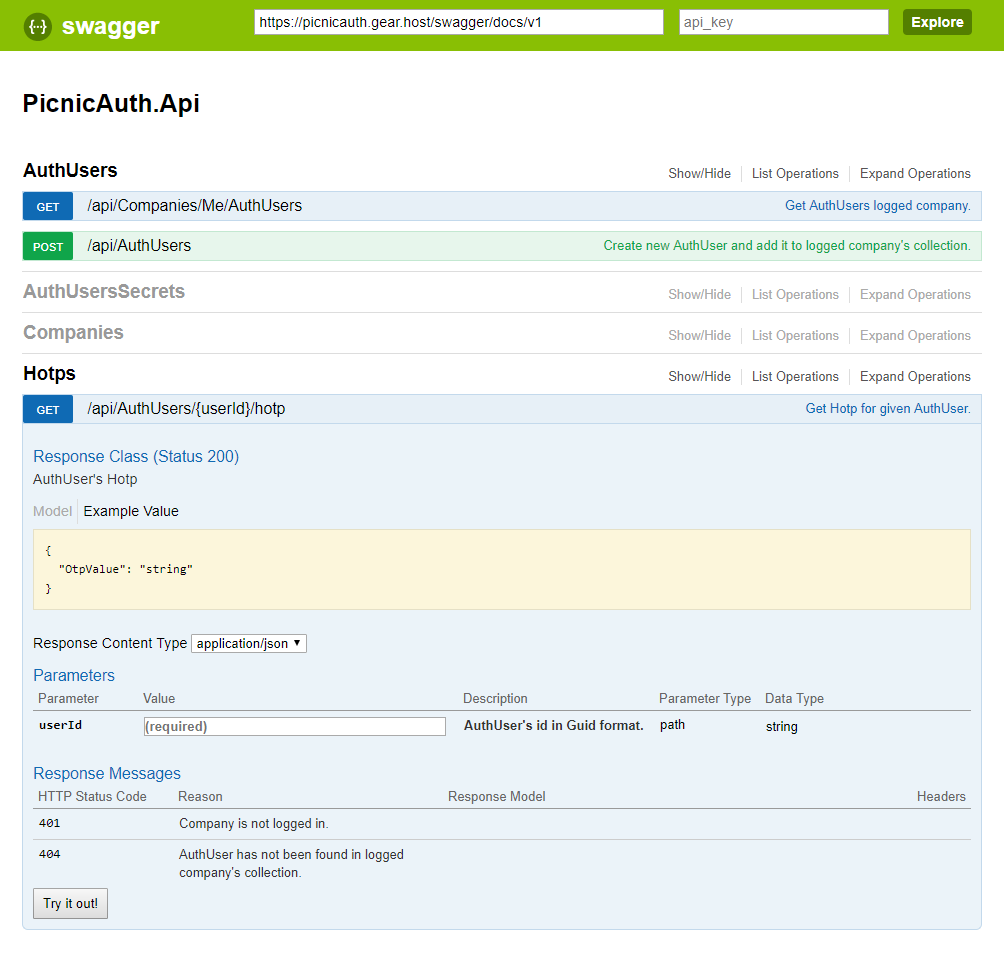
\includegraphics[width=\textwidth]{content/images/swagger}
    \caption{Interaktywna dokumentacja API.}
    \label{swagger}
\end{figure}

\subsection{Frontend}
Strona internetowa projektu (Rysunek \ref{front-home}) stworzona została w technologii \textit{Angular} w wersji~5 w konwencji 
\textit{Single Page Application}. Znajduje się na niej instrukcja użycie projektu jak również informacje
o aktualnej liczbie dostępnych bibliotek. Zawiera ona także przydatne odnośniki do repozytoriów, w których
znajduje się kod źródłowy oraz do strony na której znajduje się dokumentacja API. \\
Dodatkowymi funkcjonalnościami jakie oferuje strona jest stworzenie nowego konta dla podmiotu 
(przedstawione na Rysunku \ref{front-create}), jak również uzyskanie klucza API, 
umożliwiającego użycie bibliotek klienckich.
\begin{figure}[t]
    \centering
	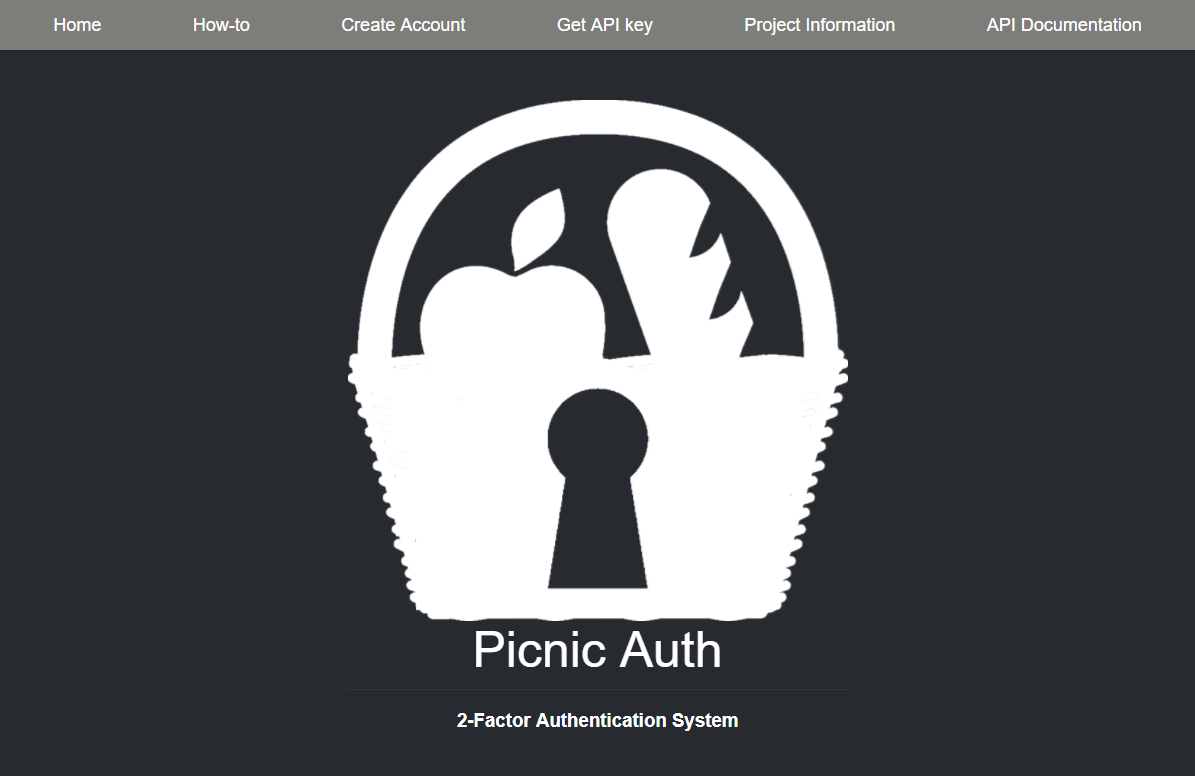
\includegraphics[width=\textwidth]{content/images/front-home}
    \caption{Informacyjna strona internetowa projektu.}
    \label{front-home}
\end{figure}
\begin{figure}[t]
    \centering
	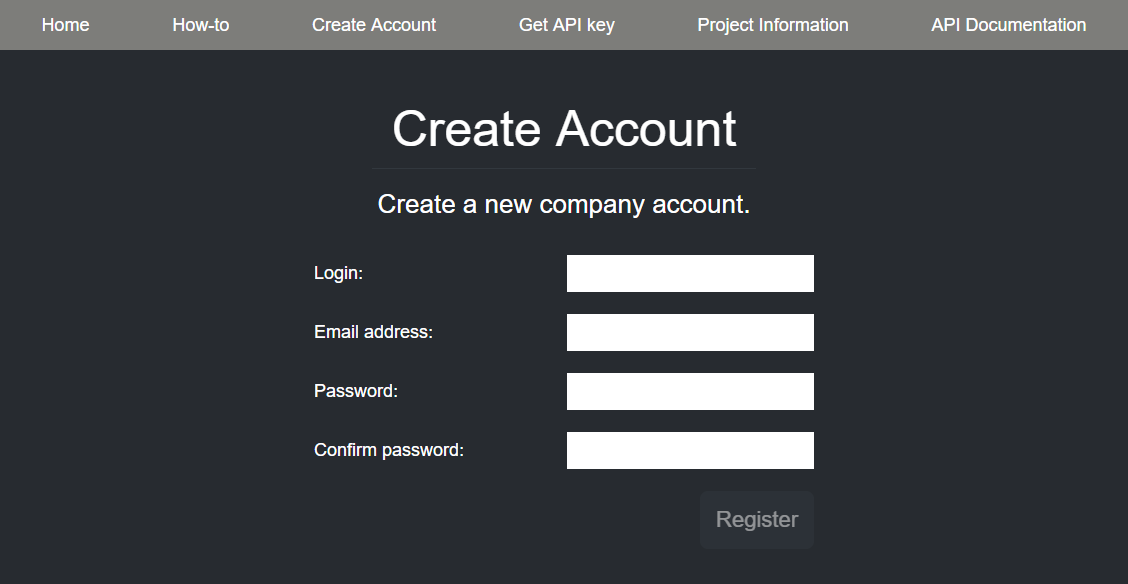
\includegraphics[width=\textwidth]{content/images/front-create}
    \caption{Tworzenie konta podmiotu.}
    \label{front-create}
\end{figure}

\subsection{Biblioteki klienckie}
W celu ułatwienia integracji z serwerem zaimplementowane zostały biblioteki klienckie.
Umożliwiają one w prosty sposób użycie funkcjonalności serwera bez konieczności 
studiowania dokumentacji i pisania kodu odpowiedzialnego za integrację. \\
Przykładowo biblioteka w języku C\# udostępnia klasę \textit{PicnicAuthClient}, posiadająca metody:
\begin{itemize}
	\item Login
	\item GetAuthUsers
	\item AddAuthUser
	\item GenereteNewSecret
	\item GetLoggedCompany
	\item AddCompany
	\item GetHotpForAuthUser
	\item ValidateHotpForAuthUser
	\item GetTotpForAuthUser
	\item ValidateTotpForAuthUser
\end{itemize}
Na chwilę obecną gotowe do użycia są biblioteki w następujących technologiach:
\begin{enumerate}
	\item C\#
	\item Visual Basic
	\item TypeScript
	\item Python 3.6
	\item Python 2.7
	\item Ruby
\end{enumerate}

\section{Tworzenie konta podmiotu}
Podmiotem jest nazywana instytucja, posiadająca użytkowników i chcąca wykorzystać w~swoim systemie 
uwierzytelnienie dwuetapowe. \\
Podmiot jest opisany bazodanowym modelem \textit{CompanyAccount}, bazującym na klasie \textit{IdentityUser}
z przestrzeni \textit{Microsoft.AspNet.Identity}.
Oprócz standardowych pól odziedziczonych z klasy \textit{IdentityUser}, model ten posiada także kolekcję 
kolekcję użytkowników \textit{AuthUser}. \\
Sam proces tworzenia nowego konta jak i autoryzacji jest zgodny ze standardowym zarządzeniem zwykłymi użytkownikami
w projekcie typu \textit{WebAPI} w technologii \textit{.Net}. \\
W~celu stworzenia nowego konta, metodą \textit{HTTP POST}, na adres \mbox{/api/Companies}, wysyłane są dane konta, 
takie jak adres poczty elektronicznej, nazwa konta oraz hasło. 
Format wysyłanych danych w postaci obiektu JSON jest przedstawiony poniżej:
\begin{lstlisting}
{
  "Email": "string",
  "UserName": "string",
  "Password": "string",
  "ConfirmPassword": "string"
}
\end{lstlisting}
Proces logowania również jest standardowy i zgodny ze standardem \textit{OAuth}.
Na adres \textit{/api/tokens}, metodą \textit{POST} wysyłane są dane takie jak nazwa konta oraz hasło
a w odpowiedzi zwracany jest token typu JWT (JSON Web Token), wykorzystywany do autoryzacji podmiotu.
Otrzymany token jest wysyłany przy każdym kolejnym zapytaniu w nagłówku w postaci \textit{Authorization: Bearer \{JWT\}}.

\section{Generacja sekretu użytkownika}
Po utworzeniu konta podmiotu możliwe jest dodanie do kolekcji użytkowników nowego użytkownika. 
Wysyłane jest wtedy zapytanie typu \textit{POST} na adres \textit{/api/AuthUsers}. Zasób pod tym adresem dostępny jest 
wyłącznie po zalogowaniu się kontem podmiotu. \\
Dane mają postać obiektu:
\begin{lstlisting}
{
  "ExternalId": "string",
  "UserName": "string",
  "Email": "string"
}
\end{lstlisting}
Po przesłaniu żądania tworzone jest konto użytkownika a następnie zapisywane jest ono do bazy. 
W procesie tym ważnym etapem jest generacja sekretu użytkownika. \\ 
Do tego celu stworzona została klasa \textit{SecureRandomNumberGenerator}, której kod widoczny jest na Rysunku \ref{code-srng}.
Wykorzystywana jest w niej klasa \textit{RNGCryptoServiceProvider} z przestrzeni \textit{System.Security.Cryptography}.
Stworzona klasa wykorzystywana jest do wygenerowania kryptograficznie bezpiecznego, pseudolosowego ciągu bajtów, zwracanego 
w formie tablicy.
\begin{figure}[t]
    \centering
	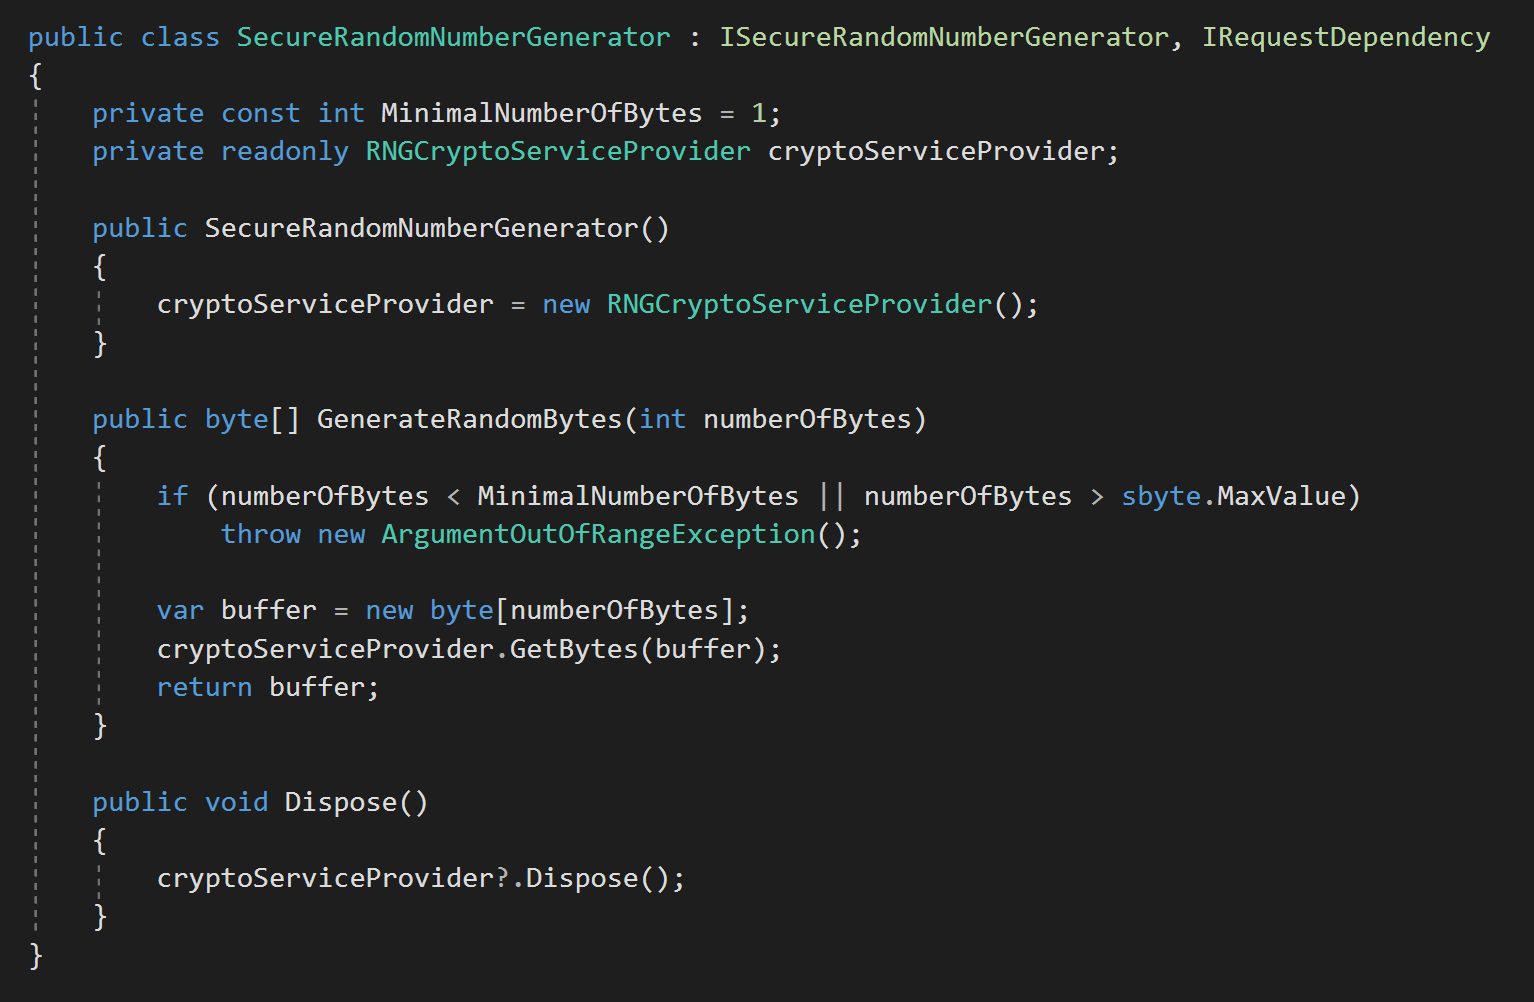
\includegraphics[width=\textwidth]{content/images/code-srng}
    \caption{Klasa zwracająca kryptograficznie bezpiecznie pseudolosowe dane.}
    \label{code-srng}
\end{figure} \\
Bardziej wyspecjalizowaną klasą jest klasa \textit{SecretGenerator}, przedstawiona na Rysunku \ref{code-secretgenerator}.
Jest w niej użyta funkcjonalność poprzedniej klasy. Zwraca ona wygenerowany sekret użytkownika, czyli ciąg bajtów o długości
zgodnej z zaleceniami standardu, równej dziesięć.
\begin{figure}[t]
    \centering
	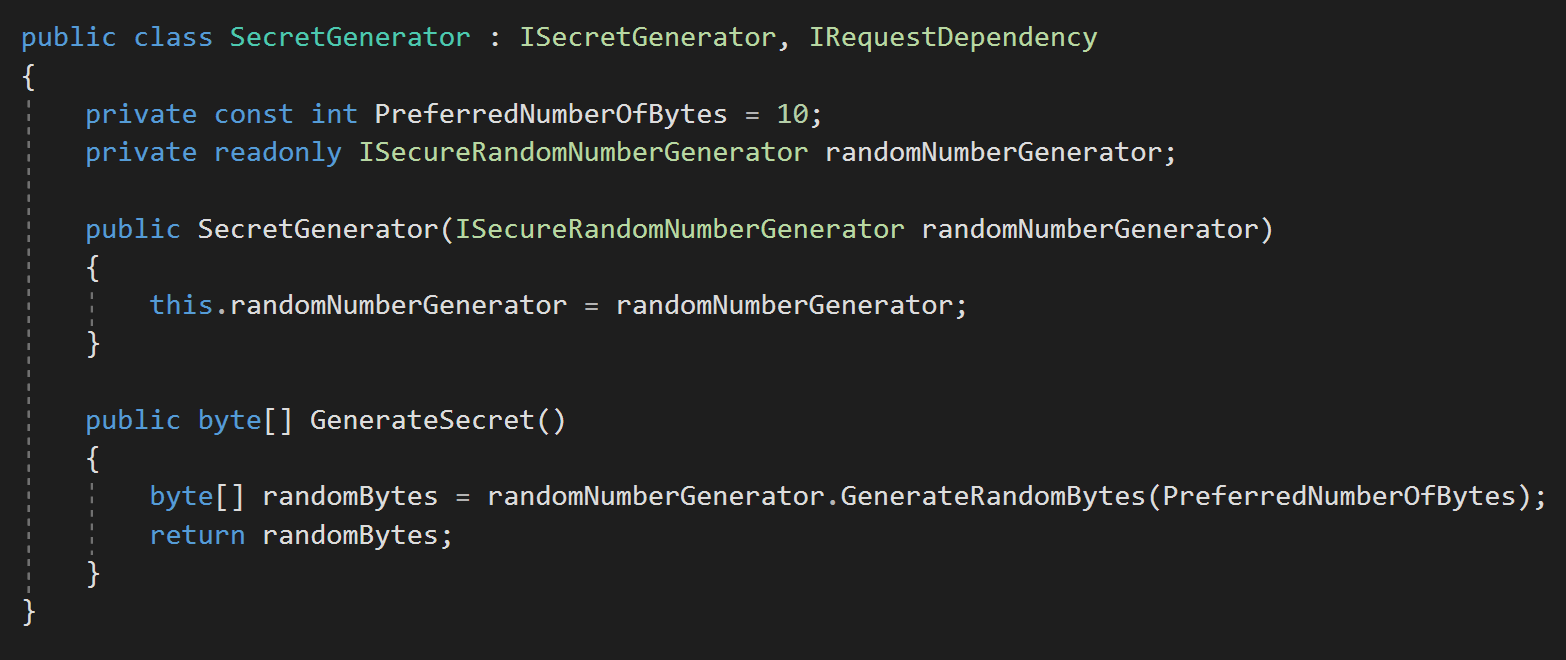
\includegraphics[width=\textwidth]{content/images/code-secretgenerator}
    \caption{Klasa generująca sekret użytkownika.}
    \label{code-secretgenerator}
\end{figure}

\section{Pobranie użytkowników powiązanych z podmiotem}
Podmiot może w dowolnym momencie uzyskać kolekcję użytkowników, których stworzył. 
Aby tego dokonać należy wysłać zapytanie na adres \textit{/api/Companies/Me/AuthUsers}. 
Zapytanie musi być typu \textit{GET} i może przyjmować parametry takie jak \textit{page} oraz \textit{pageCount}, 
wykorzystywane do paginacji. 
W przypadku niepodania któregoś z parametrów w zapytaniu przyjmują one domyślne wartości. 
Dla parametru \textit{page} domyślną wartością jest \textit{1}, a dla parametru \textit{pageCount} jest to 10. \\
Przykład zapytania z parametrami przedstawia się następująco: \\
\centerline{https://picnicauth.gear.host/api/Companies/Me/AuthUsers?page=2\&pageCount=15}

\section{Dostarczanie sekretu na urządzenie mobilne}
Po wysłaniu danych do stworzenia użytkownika w odpowiedzi wysyłany jest obiekt reprezentujący
nowo stworzonego użytkownika:
\begin{lstlisting}
{
  "ExternalId": "string",
  "UserName": "string",
  "Email": "string",
  "HotpQrCodeUri": "string",
  "TotpQrCodeUri": "string",
  "SecretInBase32": "string",
  "Id": "00000000-0000-0000-0000-000000000000"
}
\end{lstlisting}
W kwestii dostarczania sekretu użytkownika na jego urządzenie mobilne interesujące są tutaj pola
zawierające adresy do kodów QR (Quick Response) oraz pole zawierające sekret zakodowany używając kodowania transportowego \textit{Base32}.
Istnieją więc dwie metody dostarczenia sekretu. \\
Pierwsza z nich polega na przepisaniu sekretu do urządzenia mobilnego, nadaniu nazwy konta oraz wybraniu typu hasła jednorazowe.
Ekran używany do wprowadzania tych danych przedstawiony jest na Rysunku \ref{mobile-manual}.
\begin{figure}[t]
    \centering
	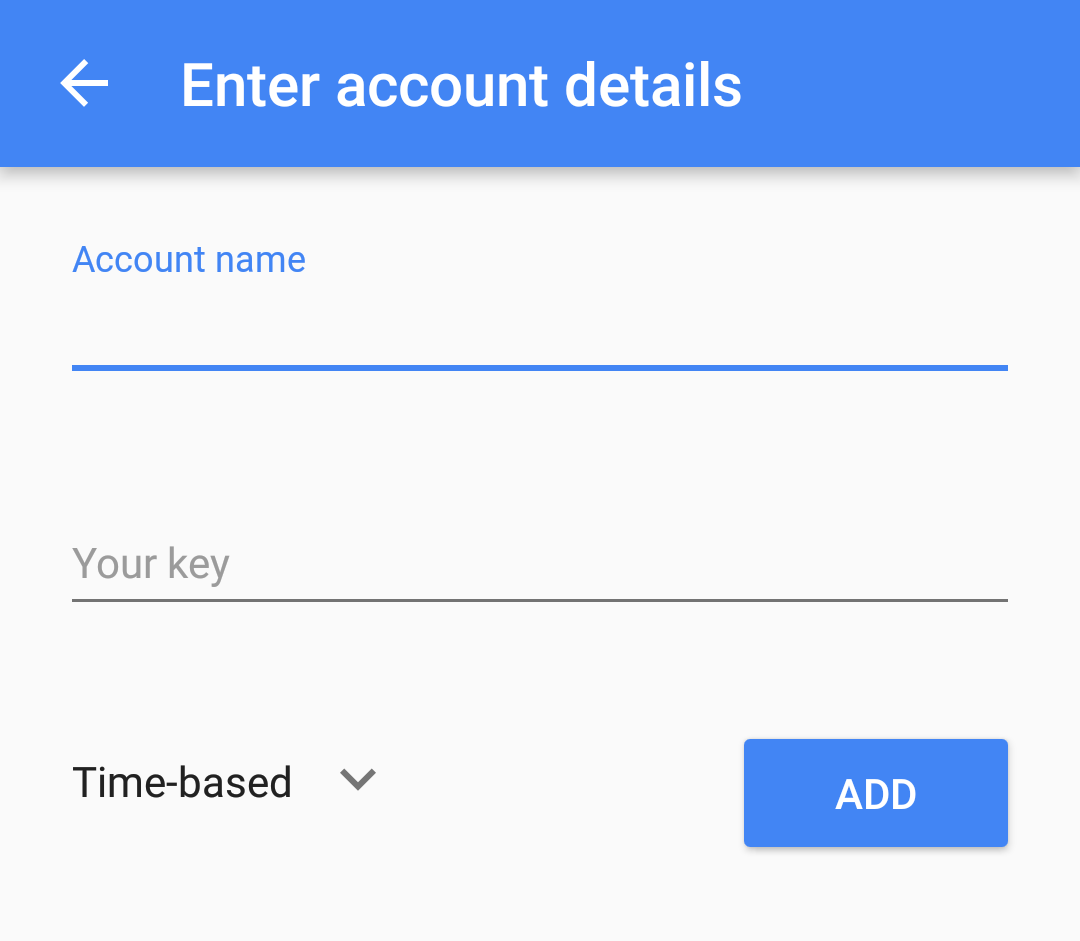
\includegraphics[width=\textwidth]{content/images/mobile-manual}
    \caption{Ekran tworzenia nowego konta w aplikacji Google Authenticator.}
    \label{mobile-manual}
\end{figure} \\
Jeśli urządzenie mobilne użytkownika jest wyposażone w aparat fotograficzny możliwe jest natychmiastowe dostarczenie sekretu, 
poprzez zeskanowanie jednego z kodów QR.
W kodach tych zakodowane są dane w formacie \textit{Key Uri}. 
Format ten jest zgodny ze standardem \textit{URI}. \\
Można go przedstawić w następujący sposób: \\
\centerline{otpauth://\{TYP\}/\{ETYKIETA\}?\{PARAMETRY\}} 
Typ może przybierać tutaj wartości \textit{hotp} lub \textit{totp}, w zależności jaki rodzaj hasła jednorazowego chcemy stosować. \\
\textit{Etykieta} używana jest do identyfikacji konta, dla którego generowane są hasła jednorazowe. 
Zwykle składa się z nazwy konta poprzedzonej nazwą podmiotu. Przykładową etykietą może być tutaj: \\
\centerline{Podmiot1:Jan.Kowalski}
Jednym z parametrów jest parametr \textit{secret}, w którym musi znajdować się sekret użytkownika zakodowany kodowaniem Base32. \\
Niewymaganym parametrem jest tutaj parametr \textit{issuer}. Jest równoznaczny z prefiksem etykiety, będącym nazwą podmiotu. 
Jeśli jest on obecny powinien przyjmować taką samą wartość jak wcześniej wspomniany prefiks. \\
Pozostałe parametry są ignorowane przez najnowszą implementację aplikacji mobilnej \textit{Google Authenticator}.
Ignorowanymi parametrami są: 
\begin{itemize}
	\item \textit{Algorithm} determinujący jaka funkcja skrótu będzie używana przy tworzeniu haseł jednorazowych. \\
		Może przyjmować wartości: 
		\begin{itemize}
			\item SHA1 (Domyślna wartość).
			\item SHA256.
			\item SHA512.
		\end{itemize}
	\item \textit{Digits} determinujący długość hasła jednorazowego. Może przyjmować wartości \textit{6} lub~\textit{8}.
		Hasło jednorazowe będzie wtedy skracane do sześciu lub ośmiu cyfr.
	\item \textit{Counter} ustalający początkową wartość licznika w przypadku haseł opartych o licznik.
	\item \textit{Period} określający okres ważności haseł opartych o czas. Domyślną wartością jest tutaj 30 sekund. 
\end{itemize}
Klasa stworzona do generacji łańcucha znaków w formacie \textit{Key Uri} przedstawiona jest na Rysunku \ref{code-keyuri}.
Wykorzystuje ona formatowanie łańcuchów znaków na podstawie z góry zadanego szablonu.
\begin{figure}[t]
    \centering
	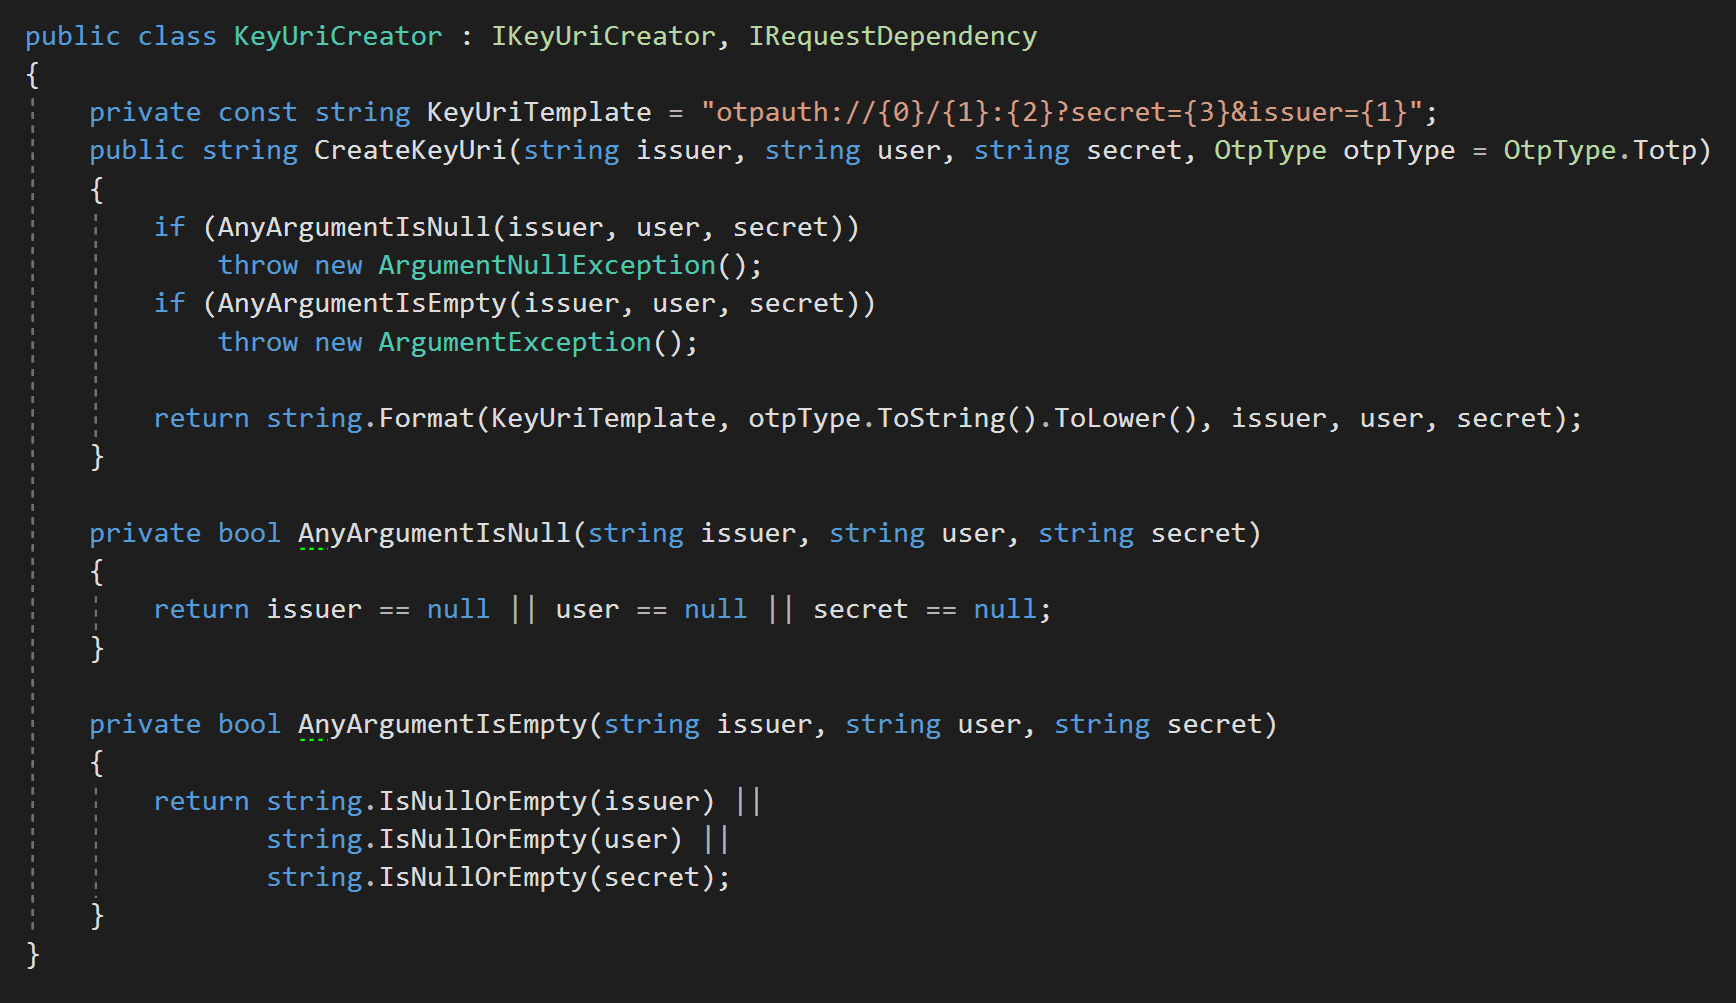
\includegraphics[width=\textwidth]{content/images/code-keyuri}
    \caption{Klasa generująca KeyUri.}
    \label{code-keyuri}
\end{figure} \\
Przykładowe kody QR o typach HOTP oraz TOTP znajdują się odpowiednio na Rysunku \ref{qr-hotp} oraz Rysunku \ref{qr-totp}.
\begin{figure}[t]
    \centering
	
\includegraphics[width=0.5\textwidth]{content/images/qr-hotp}
    \caption{Kod QR umożliwiający generację haseł typu HOTP.}
    \label{qr-hotp}
\end{figure}
\begin{figure}[t]
    \centering
	
\includegraphics[width=0.5\textwidth]{content/images/qr-totp}
	\caption{Kod QR umożliwiający generację haseł typu TOTP.}
    \label{qr-totp}
\end{figure}
Niezwykle ważne jest tutaj bezpieczeństwo samego kanału przekazywania sekretu do użytkownika końcowego. 
Konieczne jest aby cała komunikacja odbywała się z wykorzystaniem protokołu HTTPS. 
Projekt oczywiście wspiera użycie protokołu HTTPS, jak również zapobiega używaniu niezabezpieczonego kanału 
poprzez zablokowanie możliwości logowania w przypadku nieszyfrowanego połączenia.

\section{Generowanie OTP po stronie serwera}
Mając już wspólną wartość sekretu po obu stronach można przejść do procesu generacji hasła jednorazowego.
Niezależnie od wybranego typu hasła jednorazowego, wykorzystywana jest funkcja HMAC, której jednym z argumentów
jest sekret użytkownika. Klasa zaimplementowana w projekcie, wykorzystywana do uzyskania wyniku funkcji HMAC, 
przy użyciu funkcji skrótu SHA1 przedstawiona jest na Rysunku \ref{code-hmac}. \\
W implementacji tej argument \textit{key} jest równoznaczny z sekretem użytkownika.
\begin{figure}[t]
    \centering
	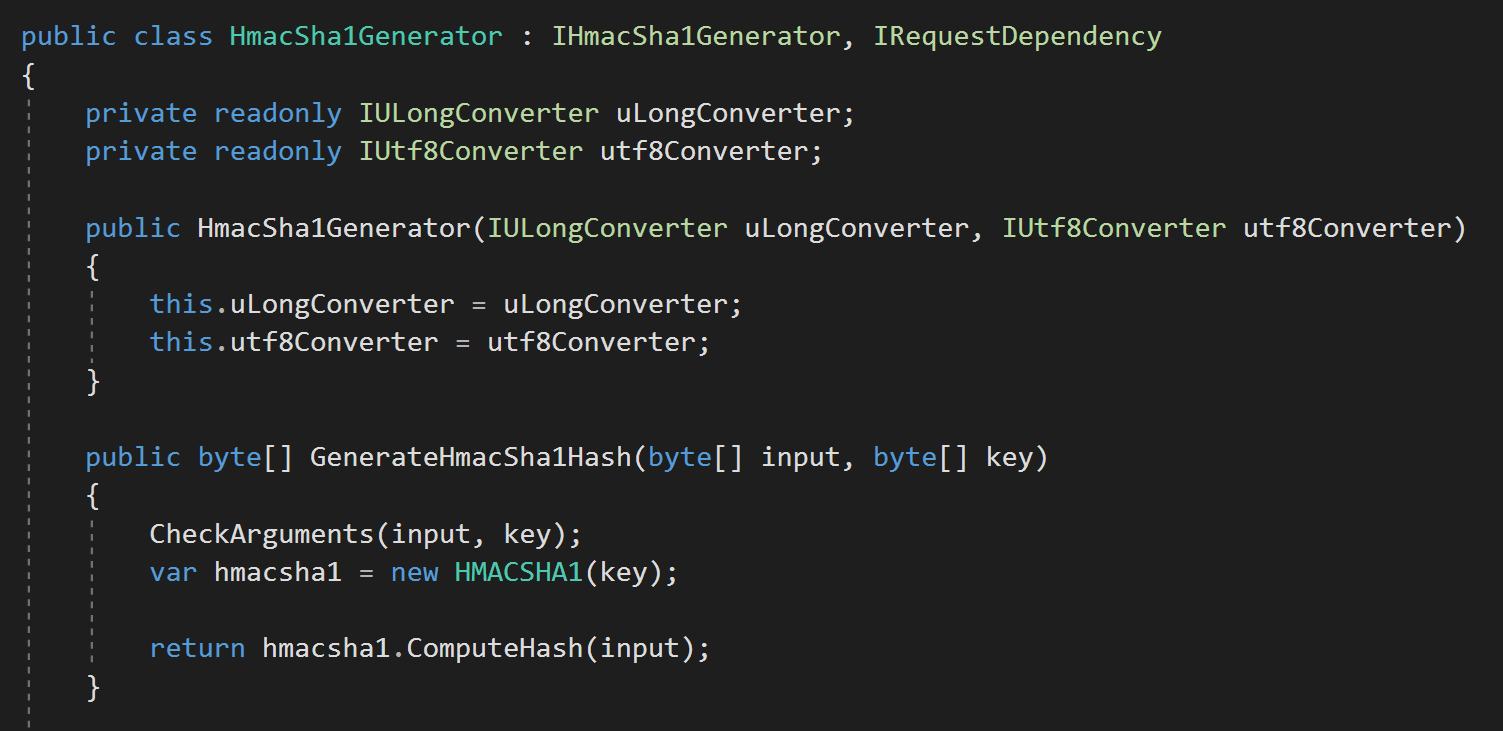
\includegraphics[width=\textwidth]{content/images/code-hmac}
    \caption{Klasa generująca HMAC.}
    \label{code-hmac}
\end{figure} \\ \\
Wynik funkcji HMAC jest następnie przycinany do postaci hasła jednorazowego. 
Hasło może zostać przycięte do sześciu lub ośmiu cyfr w zależności od preferencji podmiotu.
Sam proces przycięcia opisany został w sekcji \ref{truncate}. \\
Zaimplementowana funkcja przycinająca przedstawiona jest na Rysunku \ref{code-truncator}.
Funkcja ta pobiera wcześniej otrzymany wynik funkcji HMAC oraz liczbę cyfr, do jakiej zostanie przycięte hasło.
Domyślną liczbą cyfr, która zostanie wybrana jeśli ten argument nie zostanie podany funkcji, jest sześć. \\
Jako że prawidłową długością długością wyniku funkcji HMAC jest 20 bajtów, funkcja przycinająca sprawdza 
długość przekazanego argumentu i rzuca wyjątek w przypadku, gdy długość danych jest różna od 20 bajtów.
\begin{figure}[t]
    \centering
	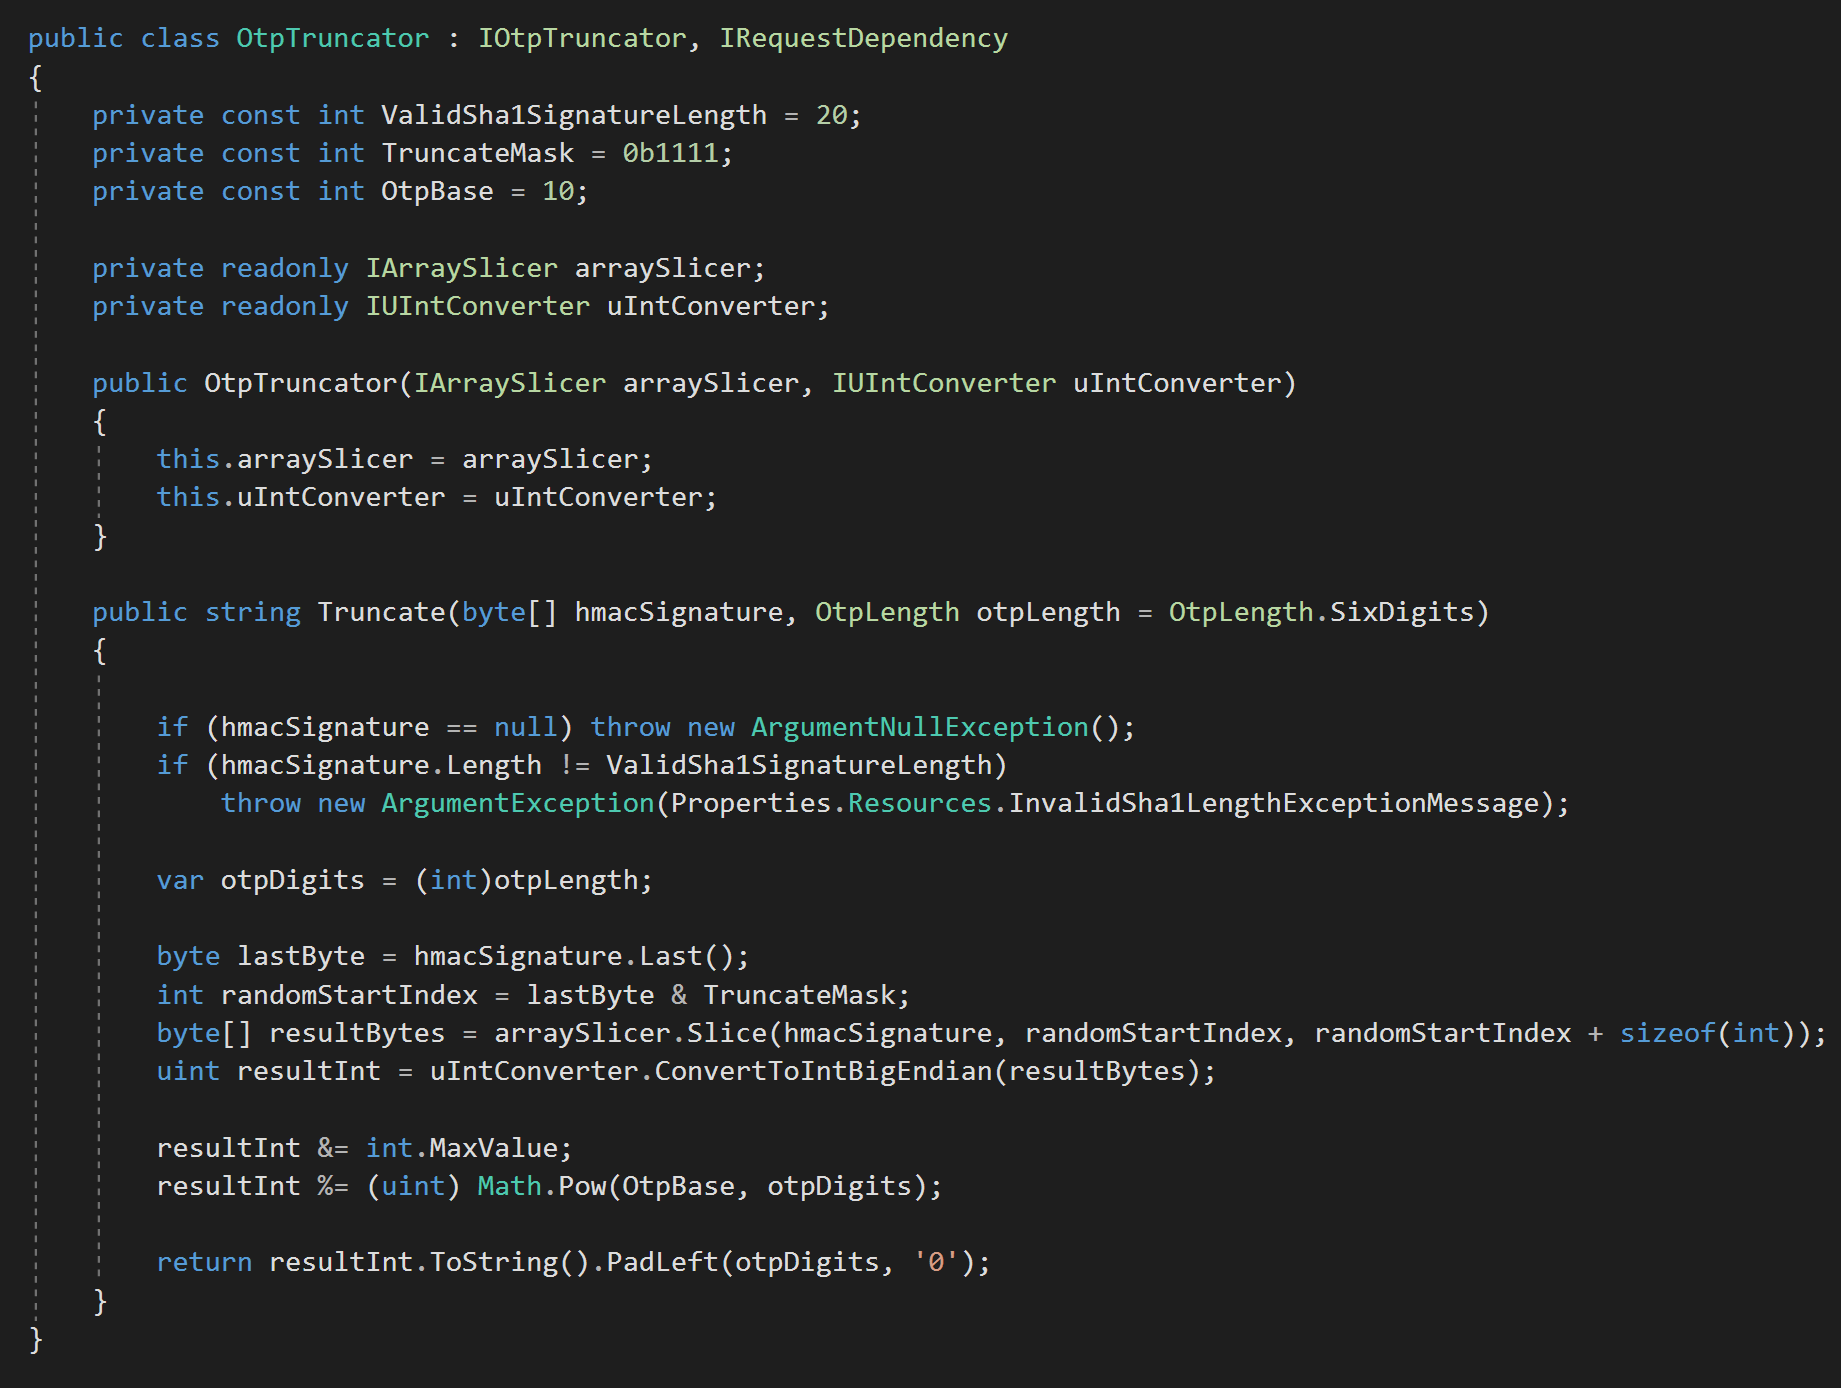
\includegraphics[width=\textwidth]{content/images/code-truncator}
    \caption{Klasa odpowiedzialna za przycięcie wyniku HMAC do postaci hasła.}
    \label{code-truncator}
\end{figure}

\subsection{Generowanie haseł typu HOTP}
Do generacji haseł typu HOTP stworzona została klasa \textit{HotpGenerator}, przedstawiona na Rysunku \ref{code-hotp}.
Funkcja \textit{GenerateHotp} w niej zawarta na podstawie licznika użytkownika oraz jego sekretu generuje hasło jednorazowe.
Funkcjonalność tej klasy bazuje na dwóch poprzednio omawianych klasach, odpowiedzialnych za wyliczenie wyniku funkcji HMAC oraz 
przycięcie wyniku funkcji HMAC do postaci hasła.
\begin{figure}[t]
    \centering
	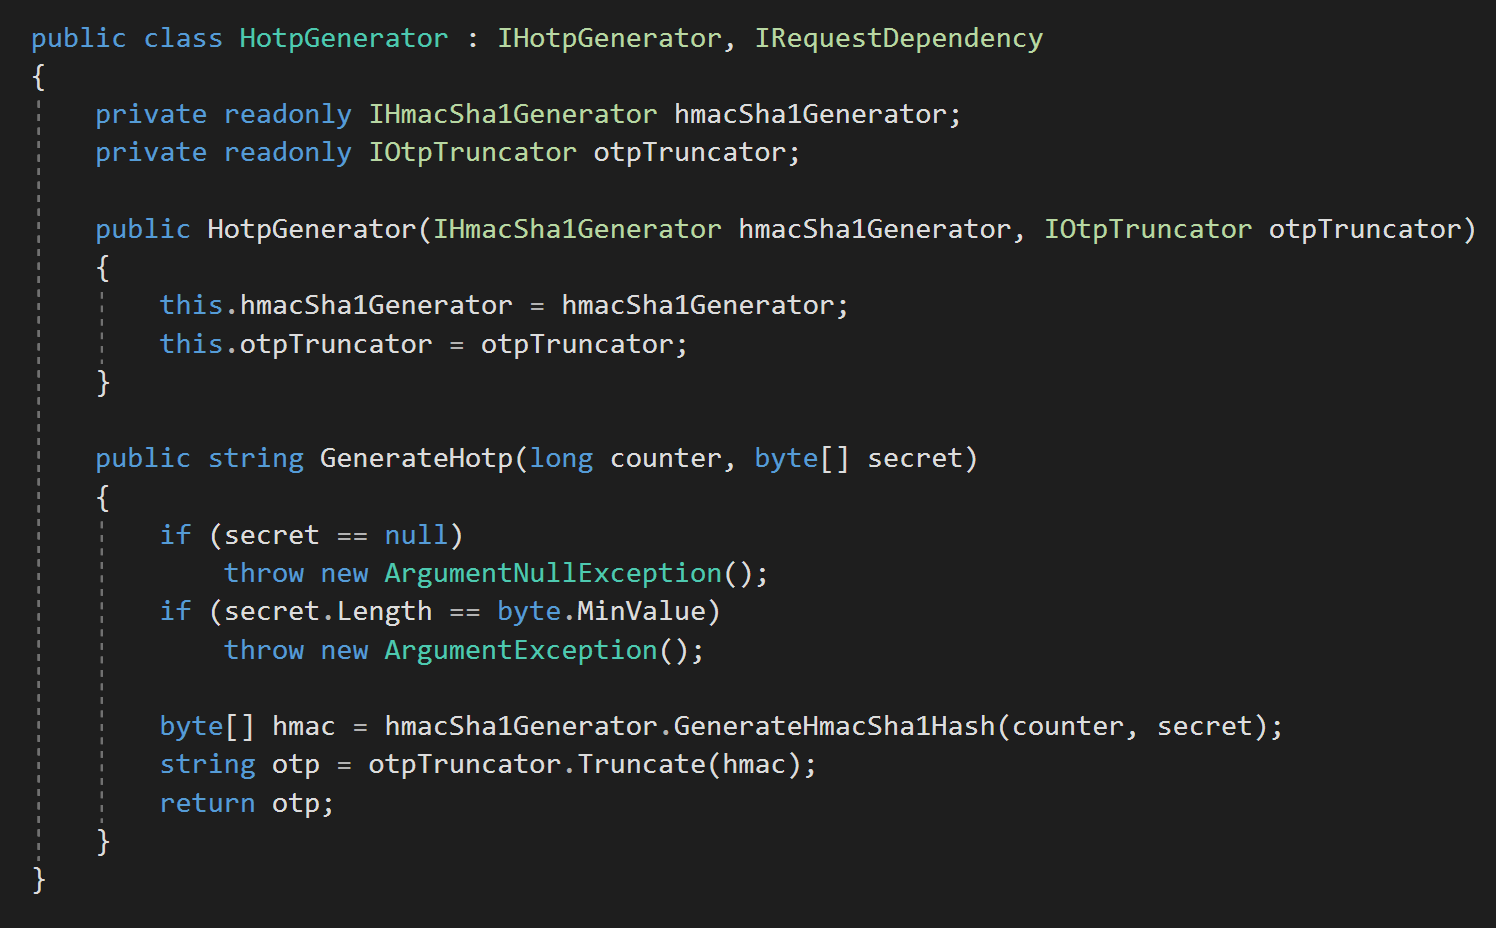
\includegraphics[width=\textwidth]{content/images/code-hotpgenerator}
    \caption{Klasa generująca hasło jednorazowe oparte o licznik.}
    \label{code-hotp}
\end{figure}

\subsection{Generowanie haseł typu TOTP}
W przypadku klasy \textit{TotpGenerator}, przedstawionej na Rysunku \ref{code-totp}, zamiast licznika, do funkcji HMAC
przekazywana jest wartość aktualnego czasu uniksowego, zwrócona przez funkcję \textit{GetUnixTimestamp}. 
Przed podaniem zmiennej \textit{currentTimestamp} do funkcji HMAC, jest ona uprzednio dzielona przez stałą 
reprezentującą okres ważności hasła jednorazowego, przyjmującą wartość zgodną ze standardem, równą trzydzieści sekund.
\begin{figure}[t]
    \centering
	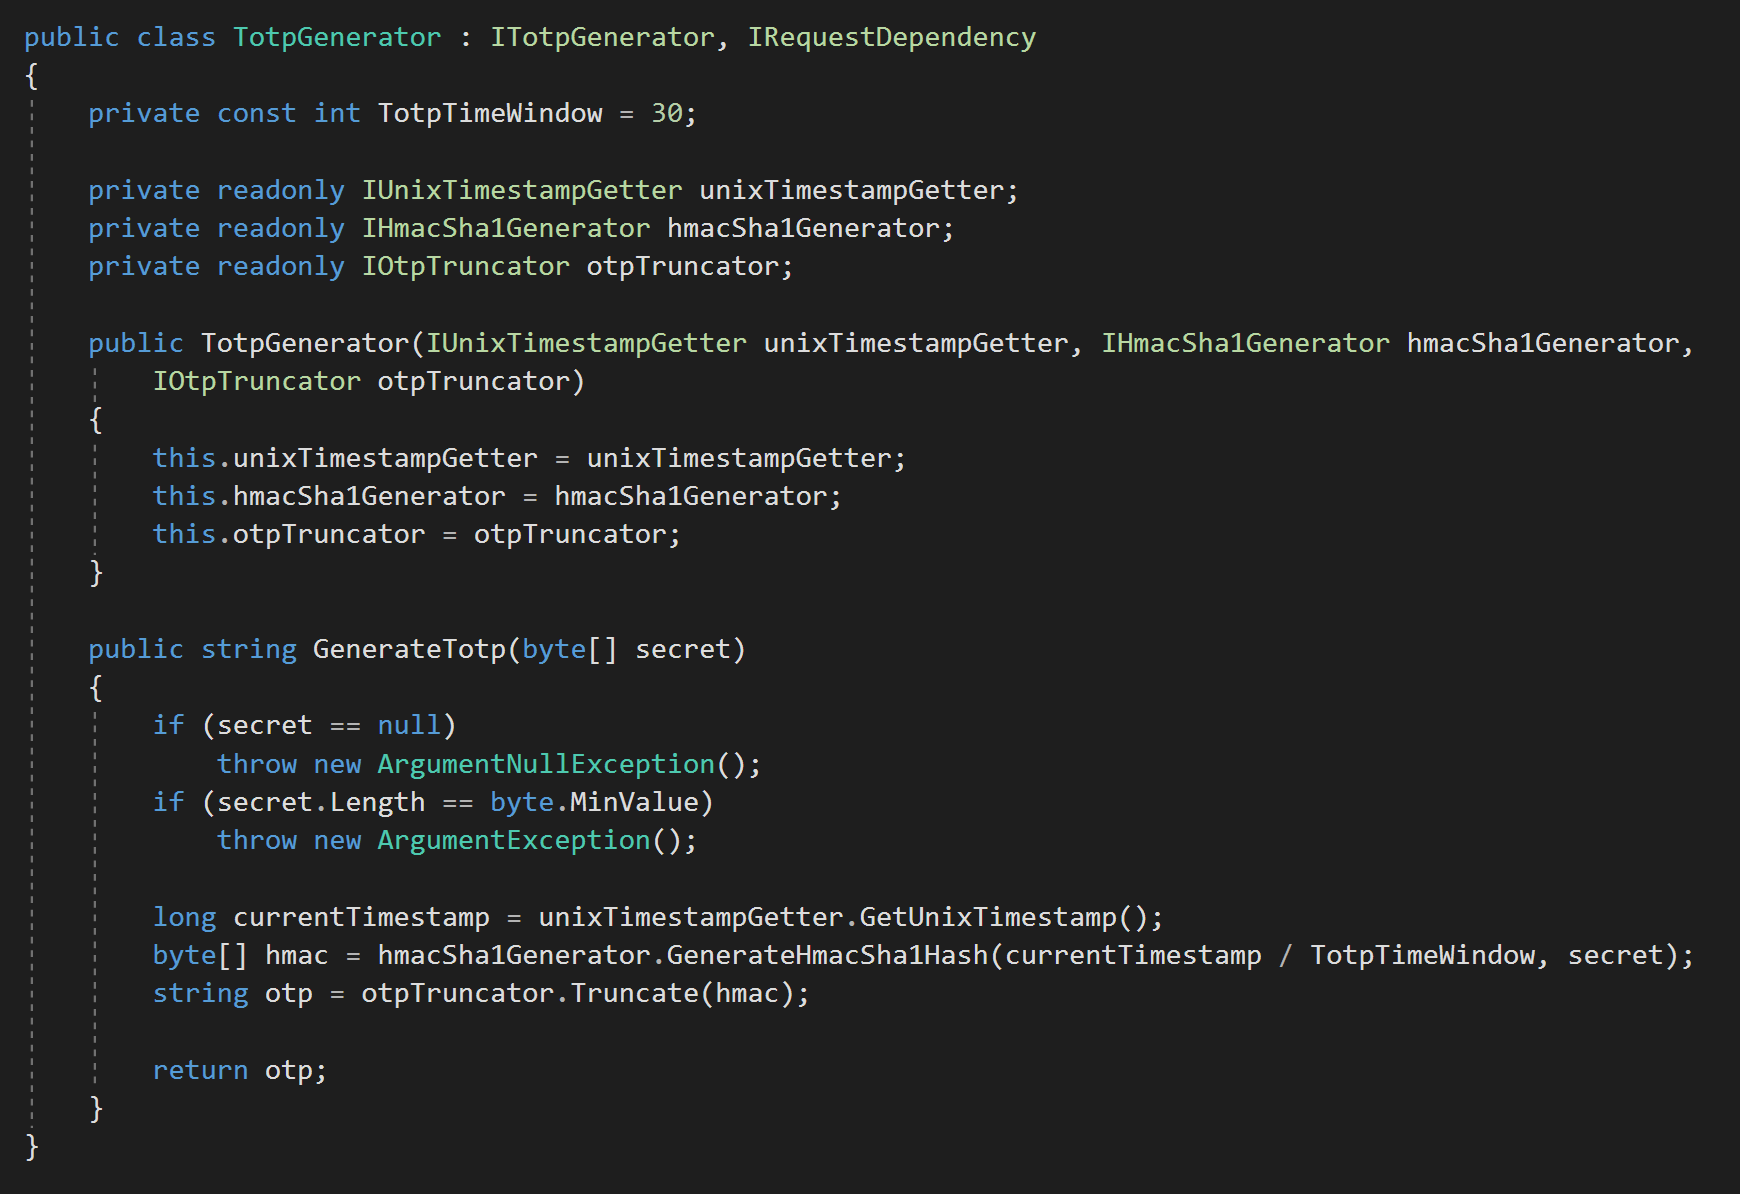
\includegraphics[width=\textwidth]{content/images/code-totpgenerator}
    \caption{Klasa generująca hasło jednorazowe oparte o czas.}
    \label{code-totp}
\end{figure}

\section{Generowanie OTP po stronie użytkownika}
Generacja haseł jednorazowych po stronie użytkownika odbywa się przy użyciu aplikacji mobilnych. 
Na tym etapie zakładamy, że sekret został już w bezpieczny sposób dostarczony na urządzenie mobilne. \\
Jedną z wielu aplikacji, których można użyć jest \textit{Google Authenticator}. 
Na Rysunku \ref{mobile-google} przedstawiony jest zrzut ekranu z tej aplikacji. 
Widnieją na nim trzy konta użytkownika, wszystkie powiązane z podmiotem \textit{sggw.pl}. 
Pierwsze od góry konto jest skonfigurowane do generacji haseł typu HOTP, opartych o licznik,
pozostałe dwa widoczne hasła, są hasłami typu TOTP, opartymi o czas uniksowy.
W celu wygenerowania kolejnego hasła typu HOTP konieczne jest na ikonę \textit{zwiniętej strzałki}.
Po kliknięciu zostanie zwiększony licznik dla tego konta a na ekranie pojawi się nowe hasło jednorazowe.
Hasła typu TOTP odświeżane są automatycznie wraz z upływem ich ważności. 
Ikona w kształcie koła, znajdująca się na prawo od hasła symbolizuje pozostały czas ważności hasła.
\begin{figure}[t]
    \centering
	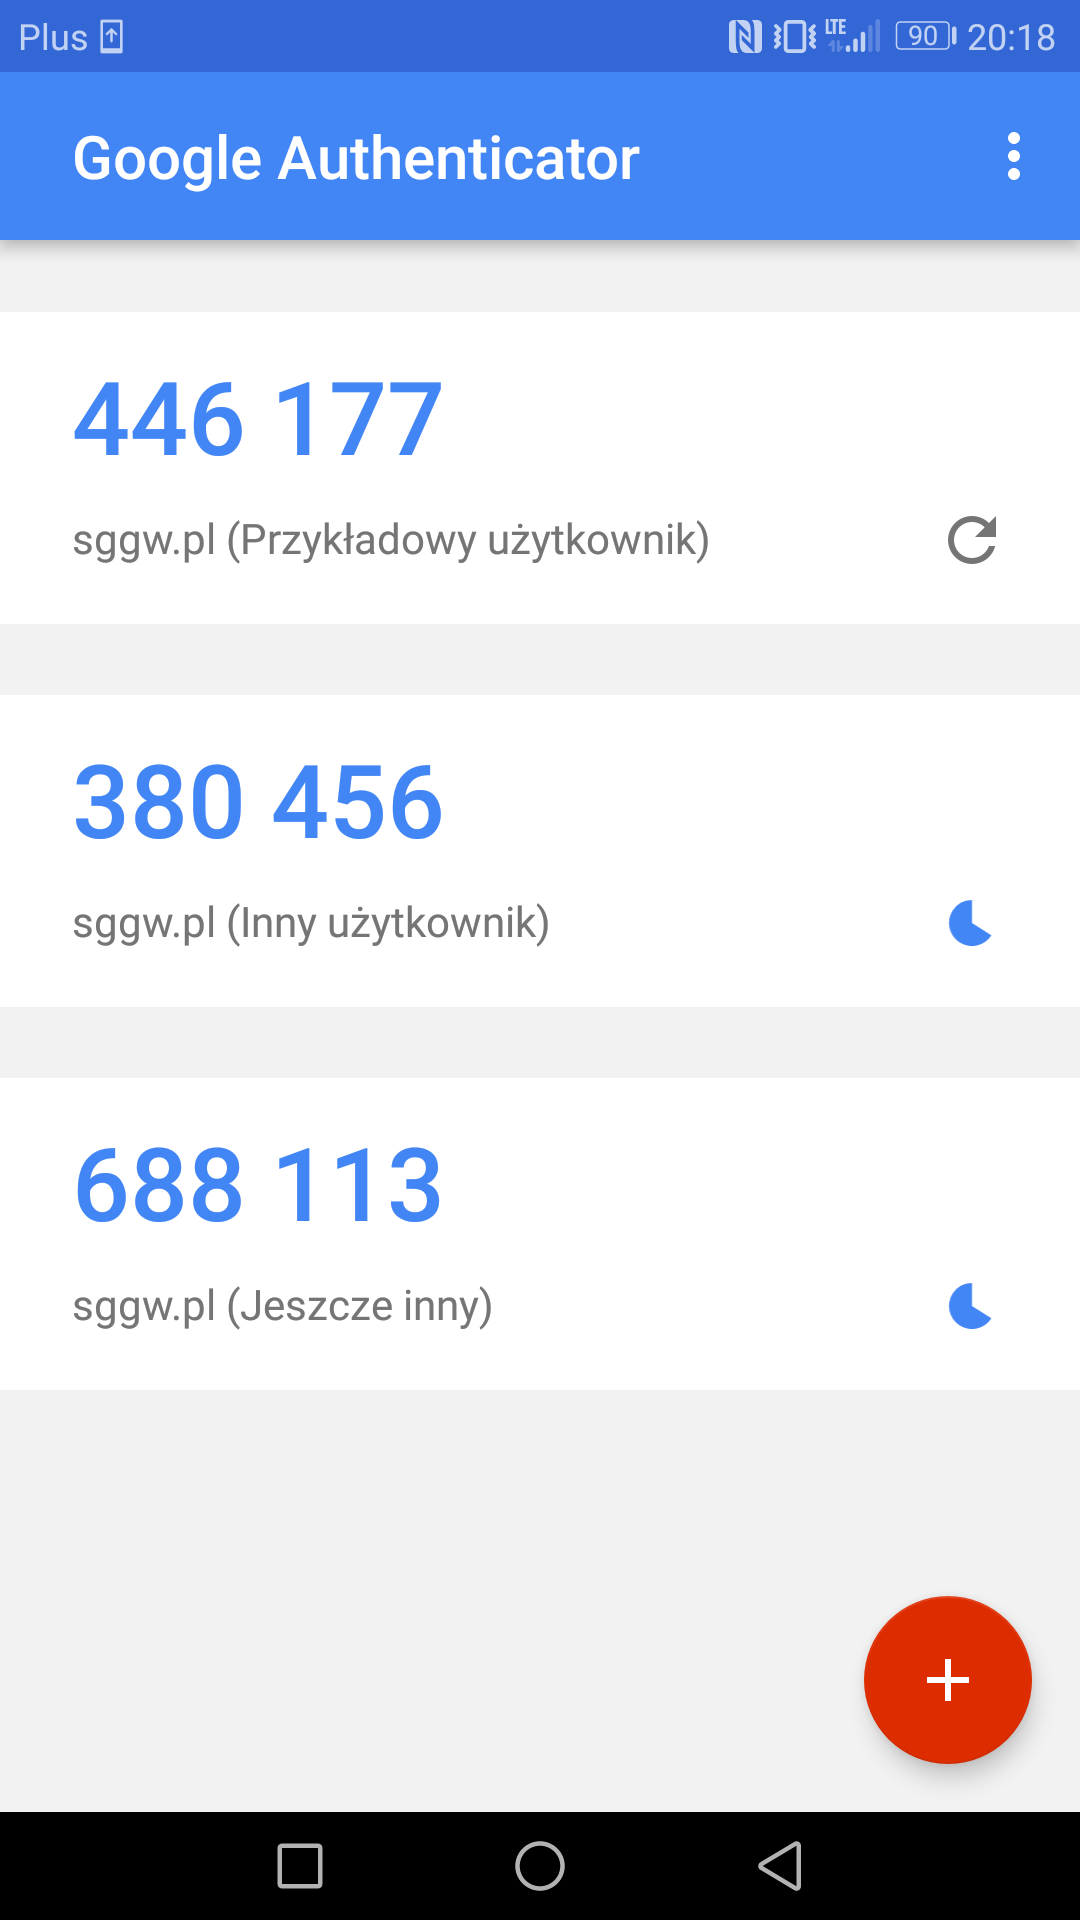
\includegraphics[width=0.5\textwidth]{content/images/mobile-google}
	\caption{Użycie aplikacji Google Authenticator.}
    \label{mobile-google}
\end{figure} \\
Bezpieczniejszą alternatywą do aplikacji \textit{Google Authenticator} jest \textit{Authy 2-Factor Authentication}. 
Posiada ona możliwość stworzenia szyfrowanych kopii zapasowych, użytecznych w przypadku zgubienia telefonu oraz
wyposażona jest w dodatkową warstwę ochrony w postaci kodu PIN, wymaganego do uzyskania haseł jednorazowych. \\
Jedną z cech podnoszących bezpieczeństwo aplikacji, odkrytych podczas testów jest zablokowana możliwość 
robienia zrzutów ekranów, jak również nagrywania ekranu z wyświetlanym hasłem jednorazowym. \\
Ekran aplikacji przedstawiony jest na Rysunku \ref{mobile-authy}. 
Widoczne jest na nim wygenerowane hasło typu TOTP dla użytkownika \textit{Przykładowy użytkownik}.
\begin{figure}[t]
    \centering
	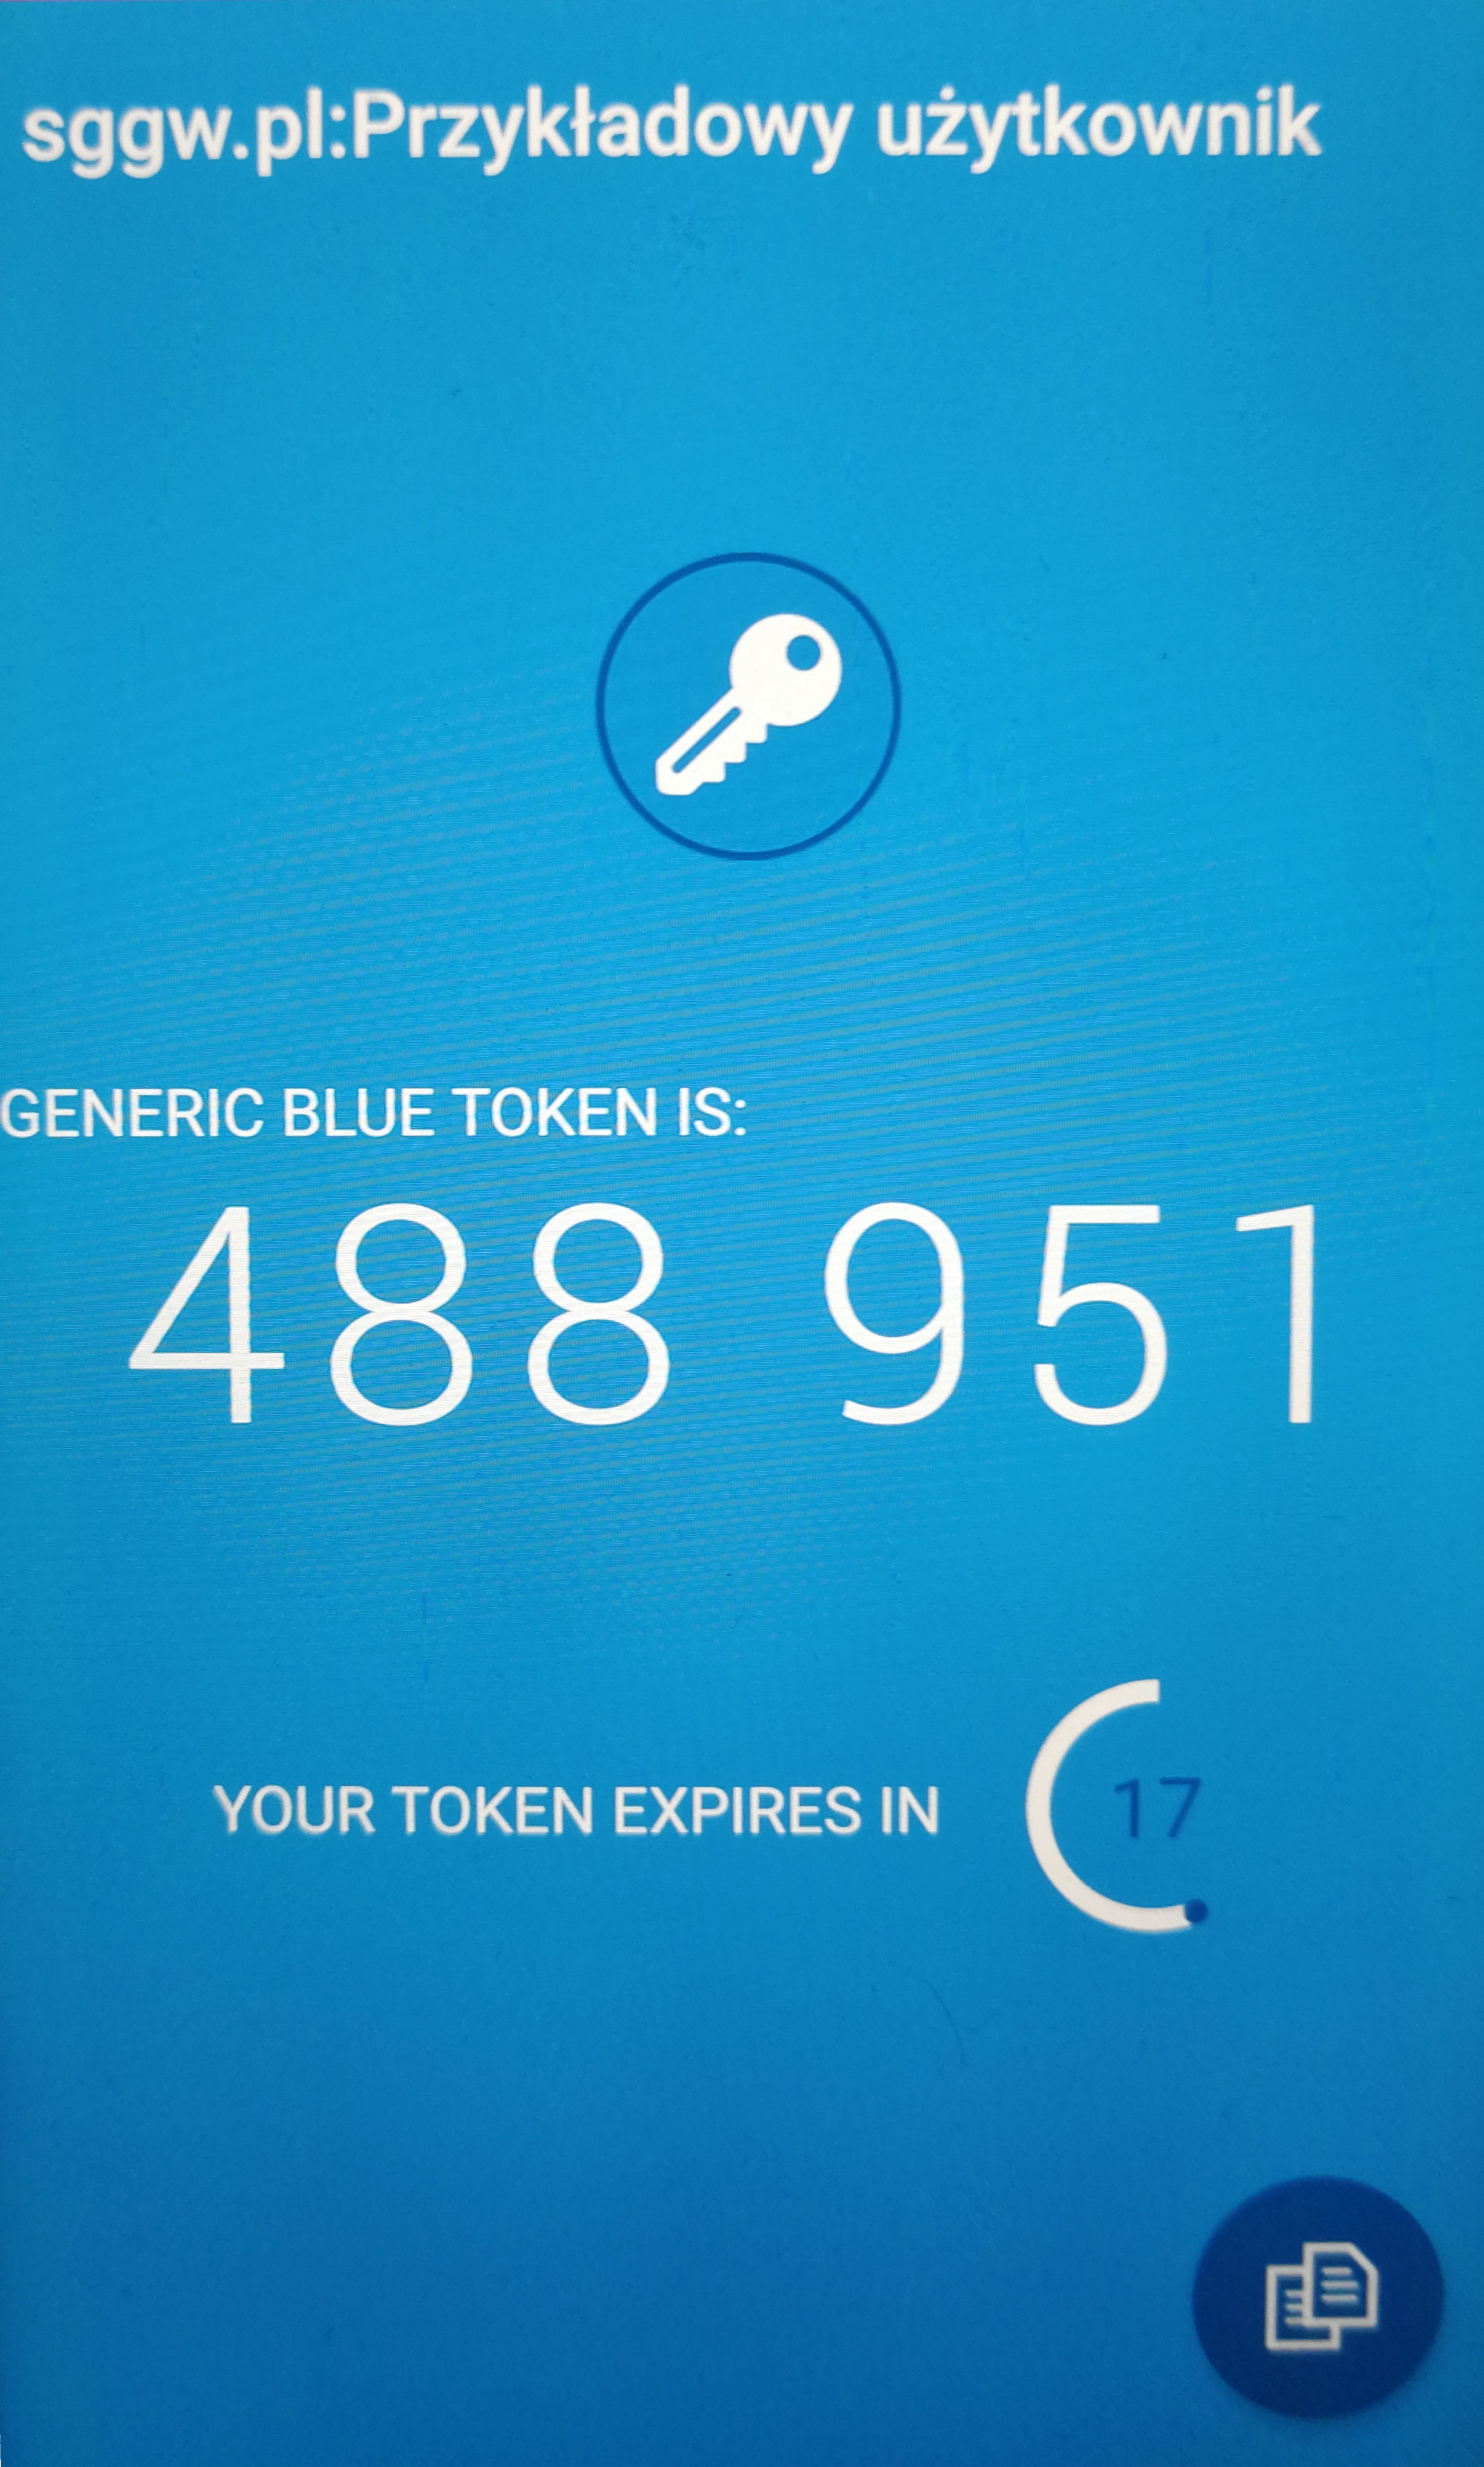
\includegraphics[width=0.5\textwidth]{content/images/mobile-authy}
	\caption{Użycie aplikacji Authy.}
    \label{mobile-authy}
\end{figure}

\section{Przechowywanie sekretu użytkownika}
Sekrety użytkowników przechowywane są w bazie danych w postaci zaszyfrowanej. 
Do konwersji sekretu użytkownika do postaci zaszyfrowanej wykorzystywany 
jest interfejs \textit{Windows Data Protection}, scharakteryzowany w sekcji \ref{wdp}. \\
Klasą odpowiedzialną za szyfrowanie sekretów użytkownika jest klasa \textit{DpapiEncryptor}, której
kod źródłowy przedstawiony jest na Rysunku \ref{code-encrypt}. Posiada ona dwie metody \textit{Encrypt}
pobierające odpowiednio tablicę bajtów oraz ciąg znaków, których można używać naprzemiennie w zależności 
od typu danych jaki chcemy zaszyfrować. Sam proces szyfrowania odbywa się \textit{w miejscu}, oznacza to że 
funkcja pobiera dane do zaszyfrowania i bezpośrednio zwraca dane w formie zaszyfrowanej, bez zapisu ich 
w~jakimkolwiek miejscu w pamięci.
\begin{figure}[t]
    \centering
	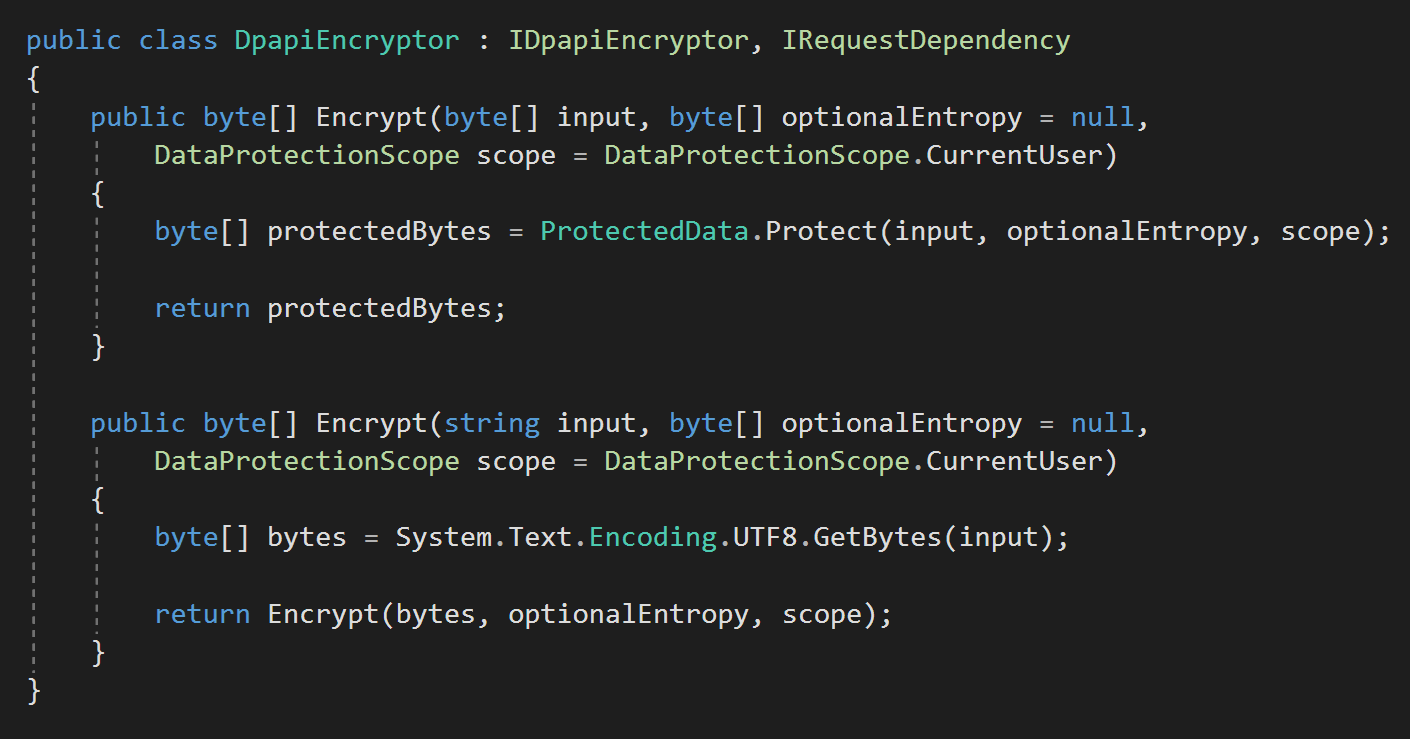
\includegraphics[width=\textwidth]{content/images/code-encrypt}
    \caption{Klasa odpowiedzialna za szyfrowanie.}
    \label{code-encrypt}
\end{figure} \\
Komplementarną do powyższej klasy jest klasa \textit{DpapiDecryptor}, przedstawiona na Rysunku \ref{code-decrypt}. 
Umożliwia ona deszyfrowanie danych, zaszyfrowanych interfejsem \textit{Windows Data Protection} do 
postaci łańcuchu znaków lub do postaci tablicy bajtów.
\begin{figure}[t]
    \centering
	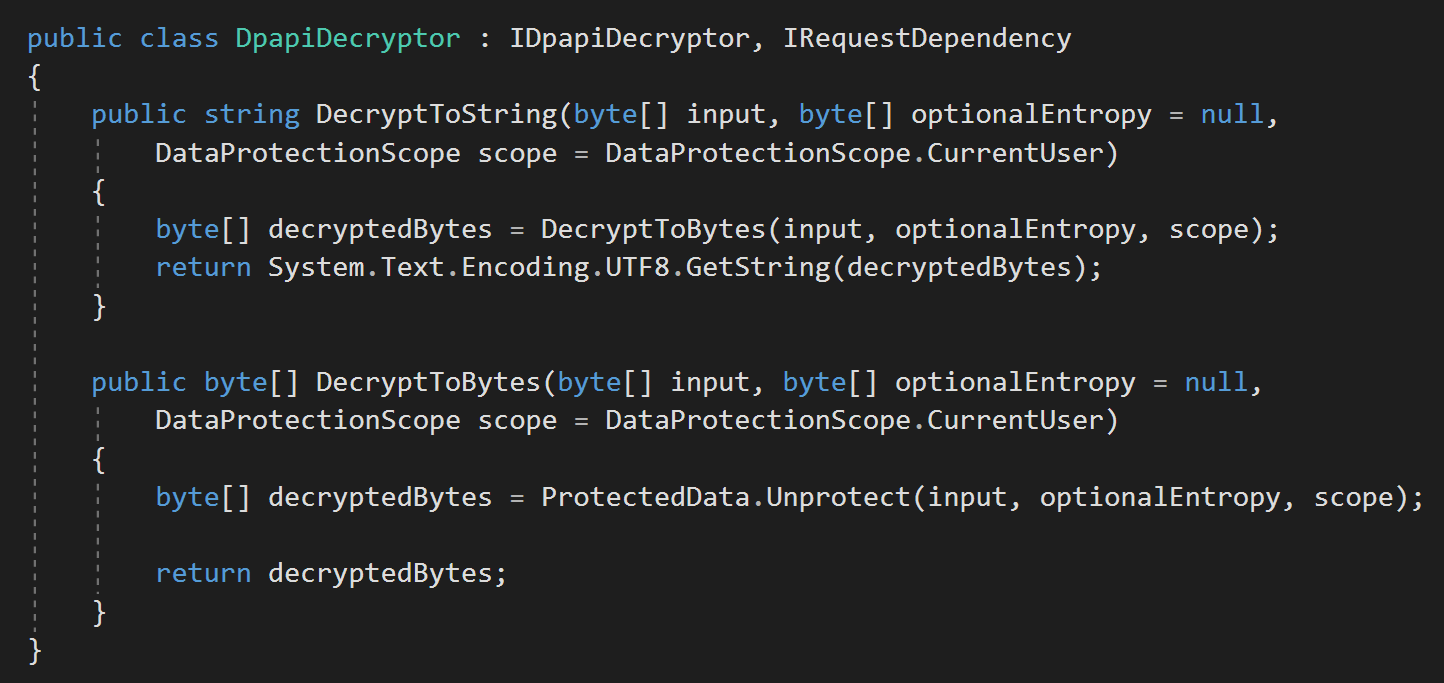
\includegraphics[width=\textwidth]{content/images/code-decrypt}
    \caption{Klasa odpowiedzialna za deszyfrowanie.}
    \label{code-decrypt}
\end{figure}

\section{Walidacja hasła jednorazowego}
W zależności od typu hasła jednorazowego proces walidacji znacząco się różni.

\subsection{Walidacja hasła opartego o licznik}
Do walidacji haseł opartych o licznik zaimplementowana została klasa \textit{HotpValidator}, której kod przedstawiony jest 
na Rysunku \ref{hotp-validator}. Posiada ona funkcjonalność walidacji pojedynczego hasła jednorazowego 
oraz kilku haseł we wcześniej skonfigurowanym przedziale. \\
W pierwszym przypadku dla podanego licznika oraz sekretu ponownie generowane jest hasło jednorazowe.
Następnie wygenerowane hasło porównywane jest z hasłem podanym przez użytkownika, jeśli obie wartości są sobie równe
zwracany wynik walidacji jest pozytywny. \\
W sytuacji, gdy użytkownik nieumyślnie kliknie na ikonę generacji nowego hasła jednorazowego 
licznik na urządzeniu przestanie być zsynchronizowany z licznikiem na serwerze. 
Przydaje się wtedy funkcjonalność walidacji w danym przydziale. 
W przypadku tego rodzaju walidacji pobierany jest z bazy obecny stan licznika. 
Jeżeli hasło wygenerowane na jego podstawie zgadza się z hasłem podanym przez użytkownika zwracany jest 
pozytywny wynik walidacji. 
W przeciwnym razie licznik jest każdorazowo zwiększany i z niego jest generowane hasło jednorazowe. 
Dzieje się tak aż do końca zadanego przedziału walidacji. 
Jeśli któreś z kolejnych wygenerowanych haseł okaże się zgodne z tym podanym przez użytkownika 
wartość licznika w bazie jest aktualizowana, tak aby była zgodna z licznikiem na urządzeniu mobilnym.
\begin{figure}[t]
    \centering
	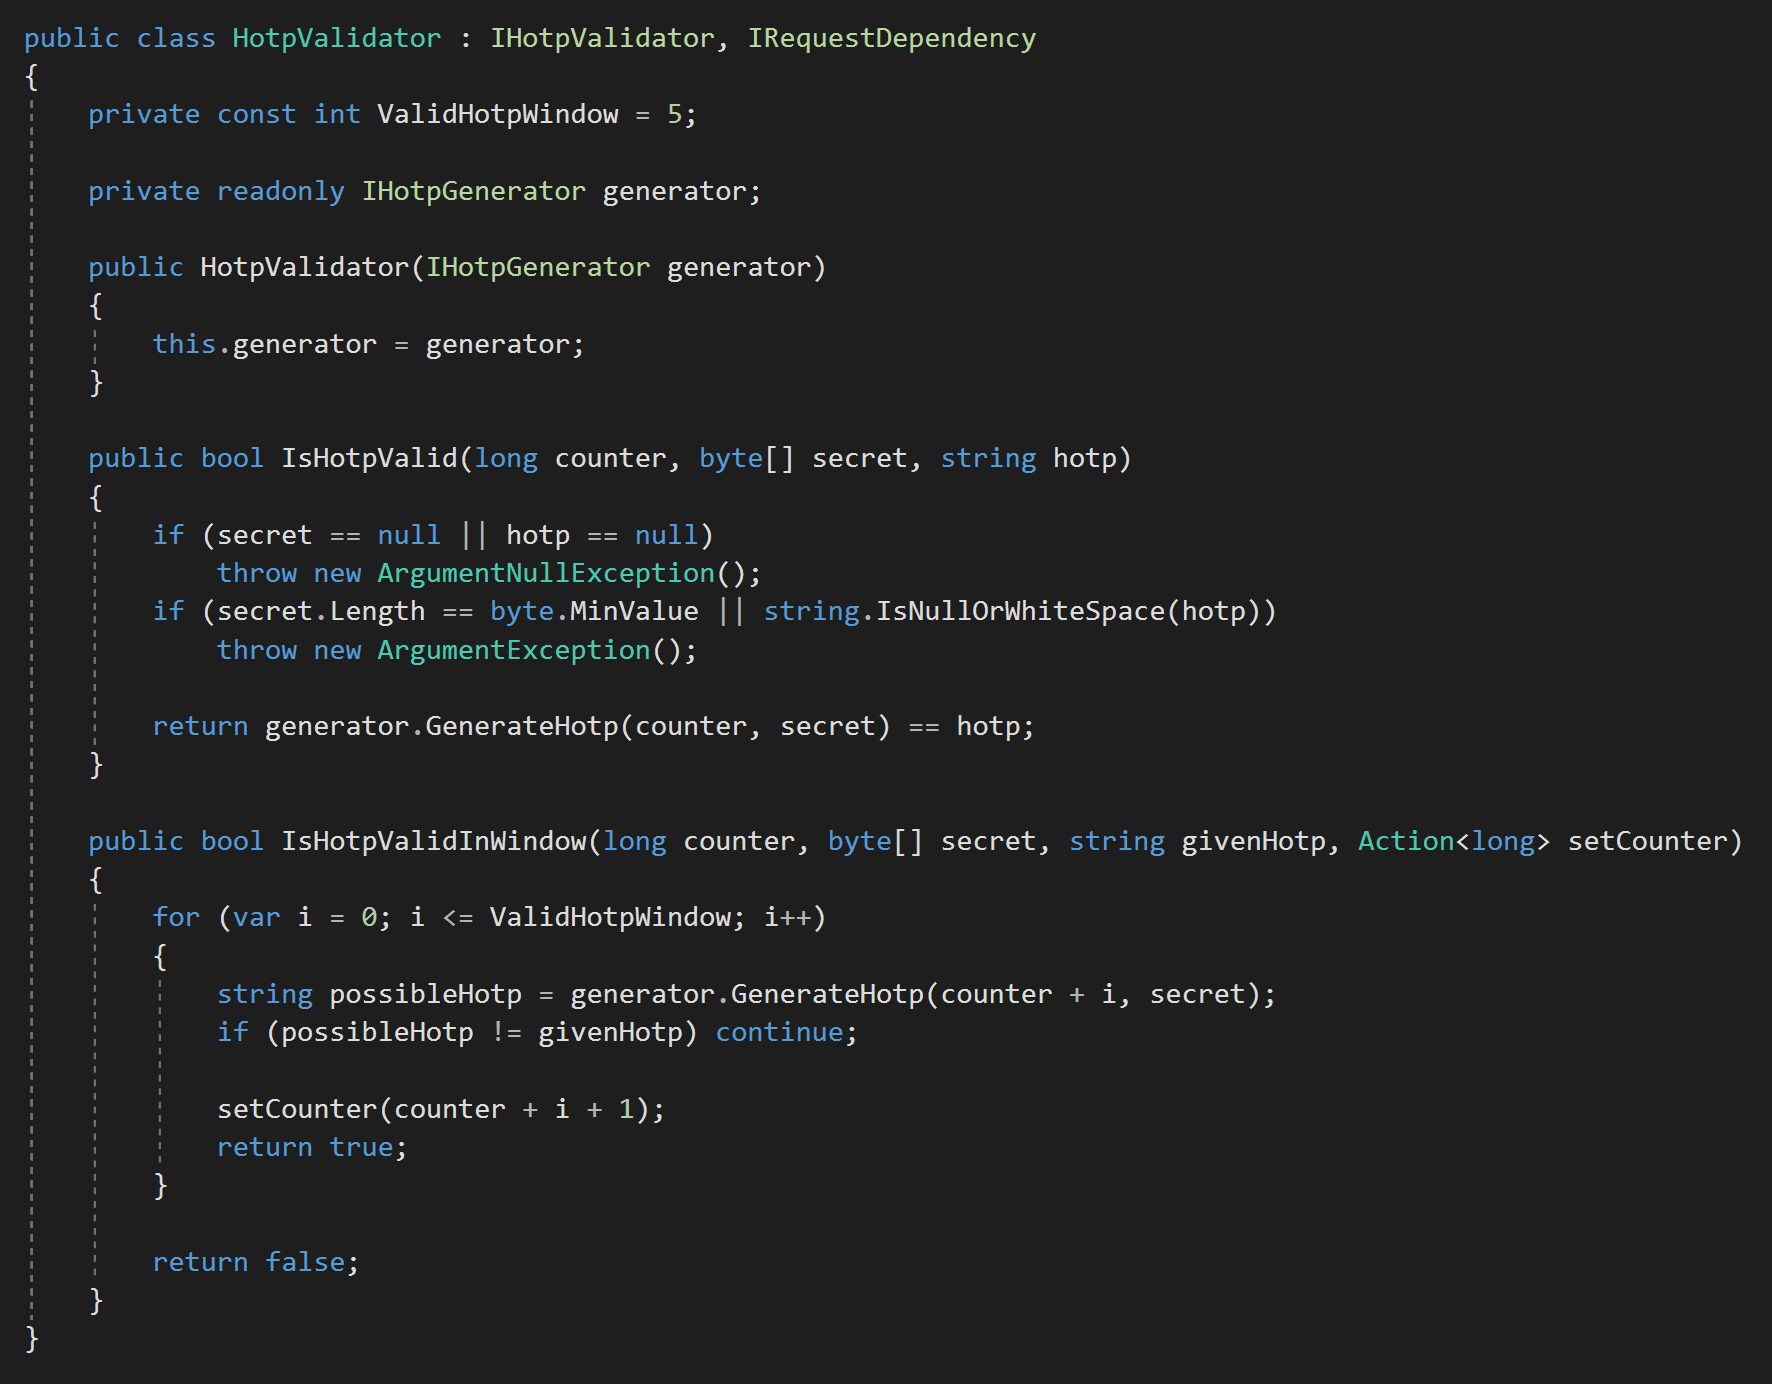
\includegraphics[width=\textwidth]{content/images/code-hvalidator}
    \caption{Klasa odpowiedzialna za walidację hasła typu HOTP.}
    \label{hotp-validator}
\end{figure} 

\subsection{Walidacja hasła opartego o czas}
Odpowiednio do walidacji haseł opartych o czas wykorzystywana jest klasa \textit{TotpValidator}, 
przedstawiona na Rysunku \ref{totp-validator}.
Z założeń obecnych w standardzie walidacja odbywa się względem trzech wartości hasła jednorazowego.
Są nimi obecna wartość hasła, poprzednia oraz następna. 
Wartości te obliczane są na podstawie czasu uniksowego podzielonego przez okno czasowe, 
czasu jedno okno czasowe wcześniej oraz czasu jedno okno czasowe później. 
Jeśli któreś z trzech wygenerowanych haseł jest zgodne z tym podanym przez użytkownika walidację można uznać za pomyślną.
\begin{figure}[t]
    \centering
	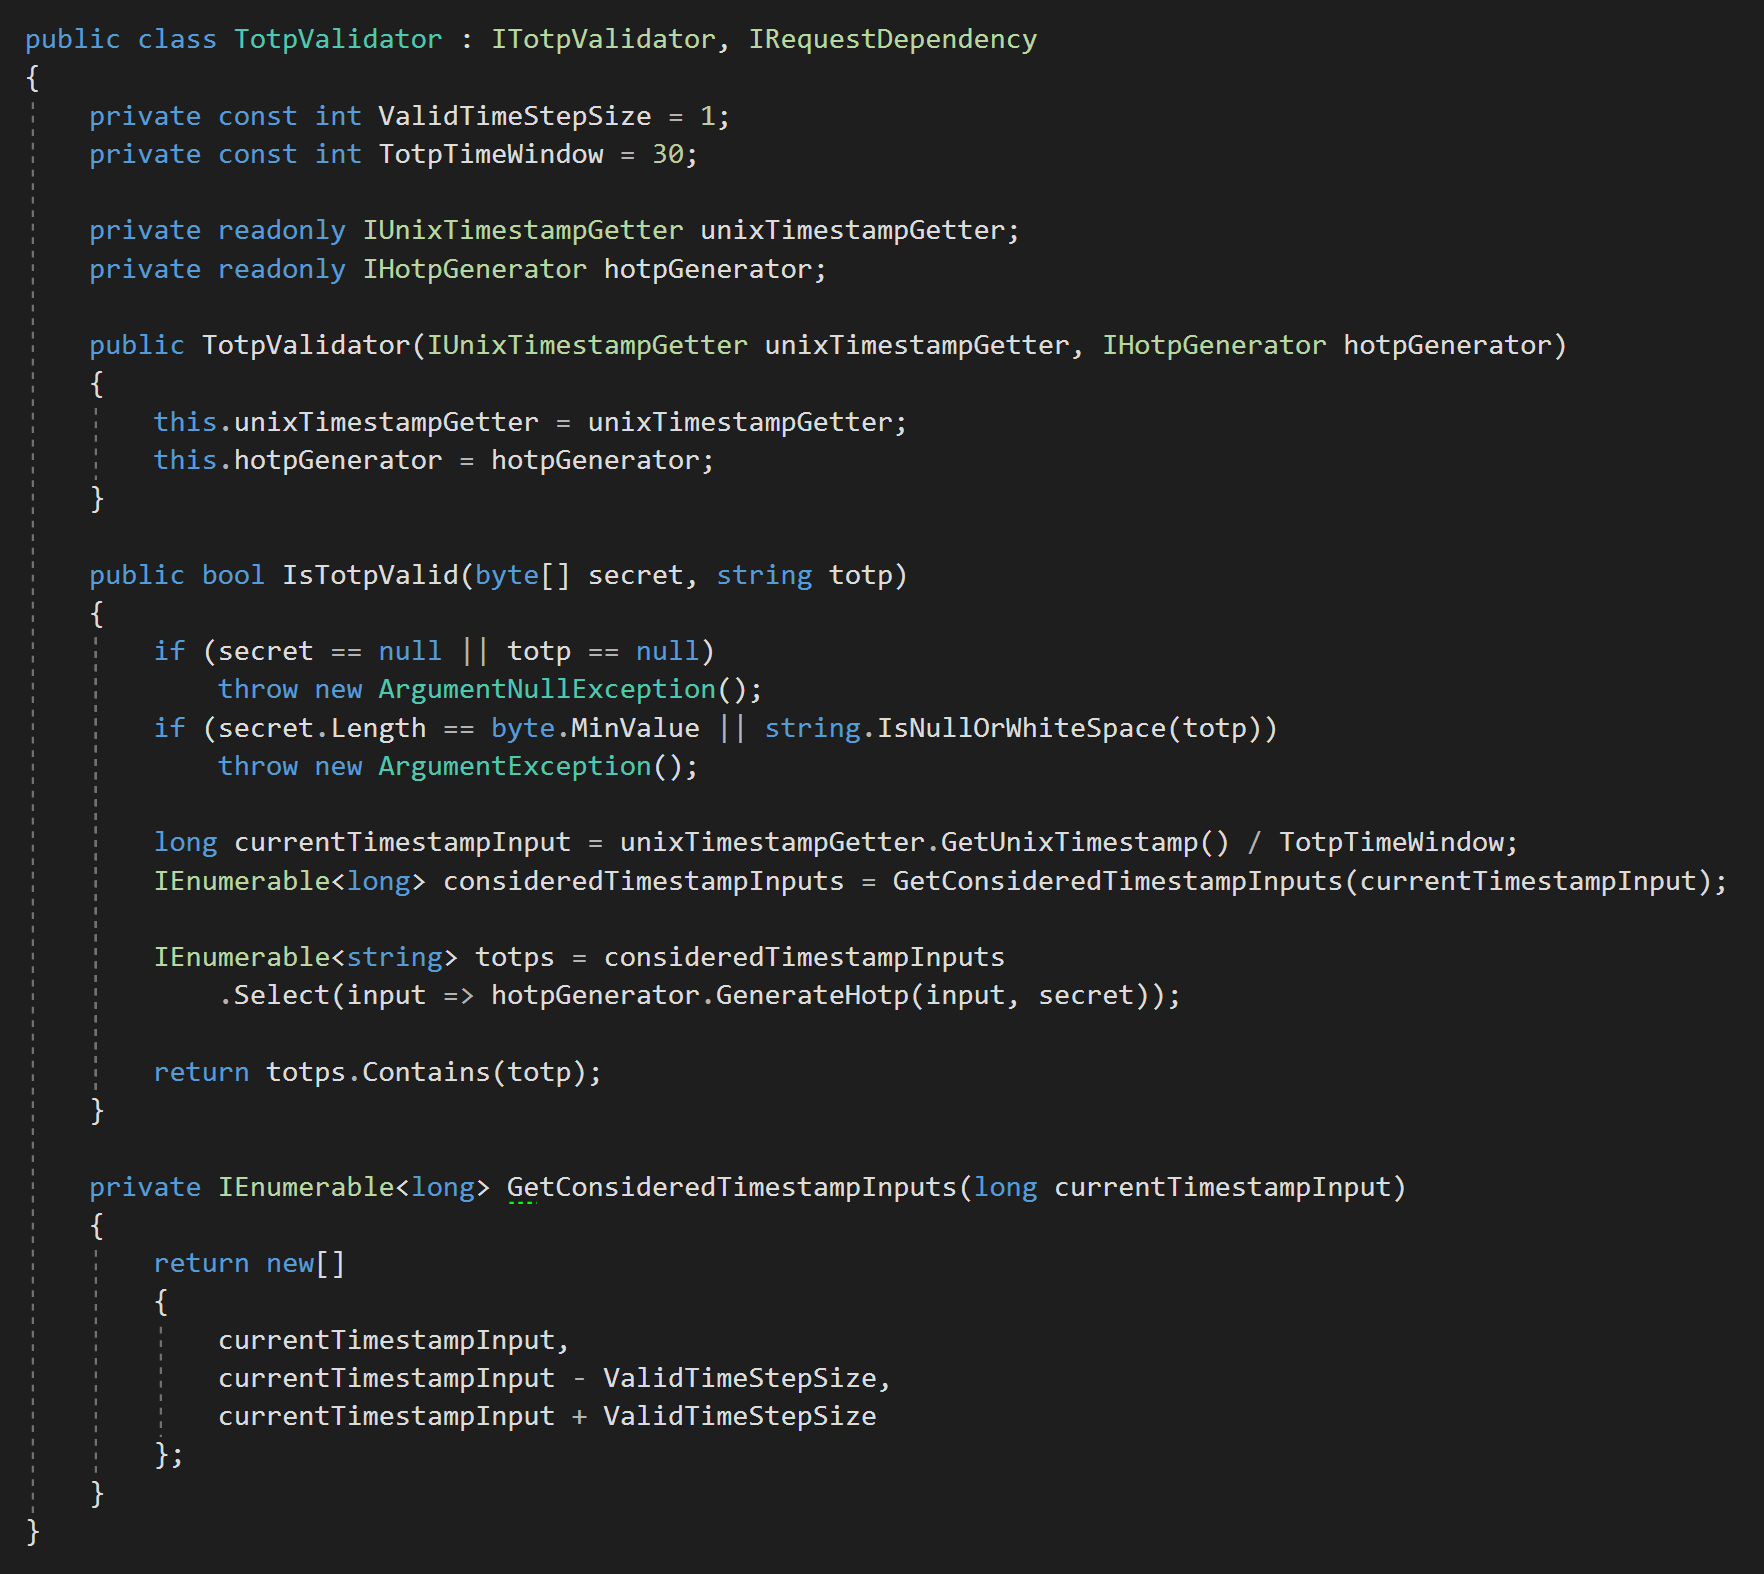
\includegraphics[width=\textwidth]{content/images/code-tvalidator}
    \caption{Klasa odpowiedzialna za walidację hasła typu TOTP.}
    \label{totp-validator}
\end{figure}

\section{Zmiana sekretu użytkownika}
Funkcjonalnością wymaganą przez standard jest generacja nowego sekretu dla użytkownika.
Jest ona konieczna w przypadku zgubienia przez użytkownika telefonu lub zdobycia jego sekretu przez osoby trzecie. \\
Aby wygenerować nowy sekret dla użytkownika wystarczy wysłać zapytanie typu \textit{PATCH} na adres: \\
\centerline{/api/AuthUsers/\{userId\}/secret}.
W zapytaniu tym za parametr \textit{userId} należy wstawić unikalny identyfikator użytkownika, któremu chcemy zmienić sekret.
Serwer zwraca obiekt JSON reprezentujący zmodyfikowanego użytkownika. 
Postać tego obiektu jest identyczna jak w przypadku procesu tworzenia nowego użytkownika.

\section{Przykład użycia projektu}
Najbardziej ogólny przypadek użycia projektu można przedstawić w następujących krokach:
\begin{enumerate}
	\item Podmiot tworzy nowe konto. \\ 
		Może to uczynić w jeden ze sposobów:
		\begin{itemize}
			\item Za pomocą strony internetowej projektu.
			\item Za pomocą interaktywnej dokumentacji API.
			\item Używając jednej z bibliotek klienckich.
			\item Wysyłając zapytanie HTTP w dowolnym języku programowania.
		\end{itemize}
	\item Pozyskanie klucza API. Sposoby równoznaczne z tymi powyżej.
	\item Wybranie jednej z bibliotek lub wysyłanie zapytań w dowolnym innym języku, w którym nie powstała jeszcze biblioteka kliencka.
	\item W sytuacji, gdy dany użytkownik chce skorzystać podmiot w systemie PicnicAuth dodaje nowego użytkownika do swojej kolekcji.
	\item Użytkownikowi przesyłany jest kod QR lub sam sekret zakodowany w Base32.
	\item Użytkownik wprowadza na swoje urządzenie mobilne otrzymany sekret.
	\item Od tej pory, gdy użytkownik chce się zalogować lub wykonać akcję o podwyższonym poziomie bezpieczeństwa, 
		wraz ze zwykłym hasłem proszony jest także o podanie hasła jednorazowego.
	\item Podmiot po otrzymaniu hasła wykorzystuje walidację w systemie PicnicAuth i w zależności od jej wyniku 
		autoryzuje próbę logowania użytkownika lub też nie.
\end{enumerate}

\section{Planowane ulepszenia}

\subsection{Generowanie hasła po stronie użytkownika}
Za najbezpieczniejsza metodę generacji haseł jednorazowych po stronie użytkownika uważany jest 
token sprzętowy, zabezpieczony kodem PIN. 
Jest to dosyć kosztowna metoda ze względu na koszty produkcji takiego tokenu, jak również 
jest mało uniwersalna, gdyż zwykle token powiązany jest z pojedynczym kontem. \\
Wychodząc na przeciw tym ograniczeniom, mogą tutaj zostać zaproponowane rozwiązania 
oparte o mikrokontroler \textit{Arduino Uno} lub o mini-komputer \textit{Raspberry Pi Zero}.
Projekt ten mógłby mieć formę DIY (Do it yourself) czyli być przepisem jak z dostarczonego 
oprogramowania i części stworzyć własny token sprzętowy, mogący generować hasła jednorazowe do wielu serwisów. 
Token posiadałby ekran, na którym wyświetlane by było wygenerowane hasło jedno razowe oraz klawiaturę 
alfanumeryczną, wykorzystywaną do podawania kodu PIN oraz do dodania nowego konta do bazy tokenu.

\subsection{Biblioteki klienckie}
Użycie REST API jest możliwe w każdej technologii umożliwiającej wykorzystanie protokołu HTTP 
wraz z formatem JSON. 
Dużo wygodniejsze jest jednak korzystanie z gotowych bibliotek, stworzonych pod daną technologię. \\ \\
W tym celu, w kolejnych wersjach projektu, planowana jest implementacja bibliotek klienckich w następujących 
językach programowania:
\begin{itemize}
	\item{C}
	\item{C++}
	\item{Clojure}
	\item{D}
	\item{Elixir}
	\item{Erlang}
	\item{Groovy}
	\item{Java}
	\item{JavaScript}
	\item{Kotlin}
	\item{Nim}
	\item{Objective-C}
	\item{Perl}
	\item{PHP}
	\item{Scala}
	\item{Swift}
\end{itemize}

\subsection{Architektura}
Możliwe jest także ulepszenie architektury części REST API projektu pod kątem większego odseparowania od siebie komponentów.
Szczególnie dotyczy to odseparowania części przechowującej sekrety użytkowników i walidującej hasła jednorazowe od reszty
aplikacji. 
W~idealnym przypadku odseparowana część umieszczona by była na osobnym systemie komputerowym, bez dostępu do Internetu. 
Komunikacja z główną częścią aplikacji powinna odbywać się wtedy poprzez minimalny interfejs, pozwalający wyłącznie na 
uwierzytelnienie podmiotu oraz walidację podanego przez użytkownika hasła jednorazowego. 
Po przesłaniu podanego przez użytkownika hasła jednorazowego, 
zwrócony zostałby jedynie wynik walidacji w postaci \textit{true} lub \textit{false}.

\subsection{Konteneryzacja części serwerowej}
Poza podstawowym przypadkiem użycia opartym o REST API wystawione pod adresem \texttt{https://picnicauth.gear.host/swagger/ui/index},
nic nie stoi na przeszkodzie wykorzystaniu kodu źródłowego aplikacji i stworzenia REST API na własnym serwerze, na przykład w firmowej
sieci lokalnej. Ten sposób wykorzystania projektu może okazać się bardziej bezpieczny, jeśli jest przez dany podmiot 
umiejętnie administrowany oraz zupełnie niebezpieczny w przeciwnym przypadku. \\
Aby ułatwić procedurę wdrożenia REST API na serwer można zaproponować tutaj użycie kontenerów. 
Dzięki nim aplikacja nie jest zależna od systemu, który jest zainstalowany na serwerze a sam proces wdrożenia jej
jest niezwykle prosty i szybki.
Może zostać użyte oprogramowanie \textit{Docker}. 

\subsection{Przechowywanie sekretu}
Obecnie do szyfrowania sekretów użytkowników wykorzystywany jest interfejs \textit{Windows Data Protection}. 
Posiada on kilka wad, między innymi to, że jest silnie zależny od hasła użytkownika sytemu. 
Lepszym ale i bardziej kosztownym rozwiązaniem, byłoby użycie szyfrowania sprzętowego zamiast wspomnianego interfejsu.
